% Options for packages loaded elsewhere
\PassOptionsToPackage{unicode}{hyperref}
\PassOptionsToPackage{hyphens}{url}
%
\documentclass[
]{article}
\usepackage{amsmath,amssymb}
\usepackage{lmodern}
\usepackage{iftex}
\ifPDFTeX
  \usepackage[T1]{fontenc}
  \usepackage[utf8]{inputenc}
  \usepackage{textcomp} % provide euro and other symbols
\else % if luatex or xetex
  \usepackage{unicode-math}
  \defaultfontfeatures{Scale=MatchLowercase}
  \defaultfontfeatures[\rmfamily]{Ligatures=TeX,Scale=1}
\fi
% Use upquote if available, for straight quotes in verbatim environments
\IfFileExists{upquote.sty}{\usepackage{upquote}}{}
\IfFileExists{microtype.sty}{% use microtype if available
  \usepackage[]{microtype}
  \UseMicrotypeSet[protrusion]{basicmath} % disable protrusion for tt fonts
}{}
\makeatletter
\@ifundefined{KOMAClassName}{% if non-KOMA class
  \IfFileExists{parskip.sty}{%
    \usepackage{parskip}
  }{% else
    \setlength{\parindent}{0pt}
    \setlength{\parskip}{6pt plus 2pt minus 1pt}}
}{% if KOMA class
  \KOMAoptions{parskip=half}}
\makeatother
\usepackage{xcolor}
\usepackage[margin=1in]{geometry}
\usepackage{color}
\usepackage{fancyvrb}
\newcommand{\VerbBar}{|}
\newcommand{\VERB}{\Verb[commandchars=\\\{\}]}
\DefineVerbatimEnvironment{Highlighting}{Verbatim}{commandchars=\\\{\}}
% Add ',fontsize=\small' for more characters per line
\usepackage{framed}
\definecolor{shadecolor}{RGB}{248,248,248}
\newenvironment{Shaded}{\begin{snugshade}}{\end{snugshade}}
\newcommand{\AlertTok}[1]{\textcolor[rgb]{0.94,0.16,0.16}{#1}}
\newcommand{\AnnotationTok}[1]{\textcolor[rgb]{0.56,0.35,0.01}{\textbf{\textit{#1}}}}
\newcommand{\AttributeTok}[1]{\textcolor[rgb]{0.77,0.63,0.00}{#1}}
\newcommand{\BaseNTok}[1]{\textcolor[rgb]{0.00,0.00,0.81}{#1}}
\newcommand{\BuiltInTok}[1]{#1}
\newcommand{\CharTok}[1]{\textcolor[rgb]{0.31,0.60,0.02}{#1}}
\newcommand{\CommentTok}[1]{\textcolor[rgb]{0.56,0.35,0.01}{\textit{#1}}}
\newcommand{\CommentVarTok}[1]{\textcolor[rgb]{0.56,0.35,0.01}{\textbf{\textit{#1}}}}
\newcommand{\ConstantTok}[1]{\textcolor[rgb]{0.00,0.00,0.00}{#1}}
\newcommand{\ControlFlowTok}[1]{\textcolor[rgb]{0.13,0.29,0.53}{\textbf{#1}}}
\newcommand{\DataTypeTok}[1]{\textcolor[rgb]{0.13,0.29,0.53}{#1}}
\newcommand{\DecValTok}[1]{\textcolor[rgb]{0.00,0.00,0.81}{#1}}
\newcommand{\DocumentationTok}[1]{\textcolor[rgb]{0.56,0.35,0.01}{\textbf{\textit{#1}}}}
\newcommand{\ErrorTok}[1]{\textcolor[rgb]{0.64,0.00,0.00}{\textbf{#1}}}
\newcommand{\ExtensionTok}[1]{#1}
\newcommand{\FloatTok}[1]{\textcolor[rgb]{0.00,0.00,0.81}{#1}}
\newcommand{\FunctionTok}[1]{\textcolor[rgb]{0.00,0.00,0.00}{#1}}
\newcommand{\ImportTok}[1]{#1}
\newcommand{\InformationTok}[1]{\textcolor[rgb]{0.56,0.35,0.01}{\textbf{\textit{#1}}}}
\newcommand{\KeywordTok}[1]{\textcolor[rgb]{0.13,0.29,0.53}{\textbf{#1}}}
\newcommand{\NormalTok}[1]{#1}
\newcommand{\OperatorTok}[1]{\textcolor[rgb]{0.81,0.36,0.00}{\textbf{#1}}}
\newcommand{\OtherTok}[1]{\textcolor[rgb]{0.56,0.35,0.01}{#1}}
\newcommand{\PreprocessorTok}[1]{\textcolor[rgb]{0.56,0.35,0.01}{\textit{#1}}}
\newcommand{\RegionMarkerTok}[1]{#1}
\newcommand{\SpecialCharTok}[1]{\textcolor[rgb]{0.00,0.00,0.00}{#1}}
\newcommand{\SpecialStringTok}[1]{\textcolor[rgb]{0.31,0.60,0.02}{#1}}
\newcommand{\StringTok}[1]{\textcolor[rgb]{0.31,0.60,0.02}{#1}}
\newcommand{\VariableTok}[1]{\textcolor[rgb]{0.00,0.00,0.00}{#1}}
\newcommand{\VerbatimStringTok}[1]{\textcolor[rgb]{0.31,0.60,0.02}{#1}}
\newcommand{\WarningTok}[1]{\textcolor[rgb]{0.56,0.35,0.01}{\textbf{\textit{#1}}}}
\usepackage{longtable,booktabs,array}
\usepackage{calc} % for calculating minipage widths
% Correct order of tables after \paragraph or \subparagraph
\usepackage{etoolbox}
\makeatletter
\patchcmd\longtable{\par}{\if@noskipsec\mbox{}\fi\par}{}{}
\makeatother
% Allow footnotes in longtable head/foot
\IfFileExists{footnotehyper.sty}{\usepackage{footnotehyper}}{\usepackage{footnote}}
\makesavenoteenv{longtable}
\usepackage{graphicx}
\makeatletter
\def\maxwidth{\ifdim\Gin@nat@width>\linewidth\linewidth\else\Gin@nat@width\fi}
\def\maxheight{\ifdim\Gin@nat@height>\textheight\textheight\else\Gin@nat@height\fi}
\makeatother
% Scale images if necessary, so that they will not overflow the page
% margins by default, and it is still possible to overwrite the defaults
% using explicit options in \includegraphics[width, height, ...]{}
\setkeys{Gin}{width=\maxwidth,height=\maxheight,keepaspectratio}
% Set default figure placement to htbp
\makeatletter
\def\fps@figure{htbp}
\makeatother
\setlength{\emergencystretch}{3em} % prevent overfull lines
\providecommand{\tightlist}{%
  \setlength{\itemsep}{0pt}\setlength{\parskip}{0pt}}
\setcounter{secnumdepth}{5}
\usepackage{booktabs}
\usepackage{longtable}
\usepackage{array}
\usepackage{multirow}
\usepackage{wrapfig}
\usepackage{float}
\usepackage{colortbl}
\usepackage{pdflscape}
\usepackage{tabu}
\usepackage{threeparttable}
\usepackage{threeparttablex}
\usepackage[normalem]{ulem}
\usepackage{makecell}
\usepackage{xcolor}
\ifLuaTeX
  \usepackage{selnolig}  % disable illegal ligatures
\fi
\usepackage[]{natbib}
\bibliographystyle{plainnat}
\IfFileExists{bookmark.sty}{\usepackage{bookmark}}{\usepackage{hyperref}}
\IfFileExists{xurl.sty}{\usepackage{xurl}}{} % add URL line breaks if available
\urlstyle{same} % disable monospaced font for URLs
\hypersetup{
  pdftitle={The Revised Universal Soil Loss Equation (RUSLE) for post-fire soil erosion modelling.},
  hidelinks,
  pdfcreator={LaTeX via pandoc}}

\title{The Revised Universal Soil Loss Equation (RUSLE) for post-fire soil erosion modelling.}
\author{true}
\date{2023-02-27}

\begin{document}
\maketitle

{
\setcounter{tocdepth}{2}
\tableofcontents
}
\hypertarget{overview}{%
\section*{Project Overview}\label{overview}}
\addcontentsline{toc}{section}{Project Overview}

\hypertarget{motivation}{%
\subsection*{Motivation}\label{motivation}}
\addcontentsline{toc}{subsection}{Motivation}

Modelling soil erosion in post-burn areas is critical for understanding how broad-scale change impacts soil properties and structures. The RUSLE, the most commonly used soil erosion model, has primarily been applied to model soil erosion in agricultural regions. Applying the RUSLE in non-agriculture regions presents a substantial challenge. This challenge is driven by data availability and the applicability of RUSLE factors for non-uniform slopes and cover classes. As a result, RUSLE outcome values for non-linear, semi-natural, or steep regions must be considered the spatial representation of trends in soil erosion. In this report, we demonstrate the application of the RUSLE for modelling soil erosion across two watersheds in the Kootenay region of British Columbia. The RUSLE soil erosion maps demonstrate the spatial variation of soil erosion across the study area and signify areas where soil erosion is predicted to be higher or lower.

\hypertarget{objective}{%
\subsection*{Objective}\label{objective}}
\addcontentsline{toc}{subsection}{Objective}

This project aims to apply the Revised Universal Soil Loss Equation (RUSLE) for post-fire soil erosion modelling in a study area in the West Kootenay region of southeastern British Columbia. The specific objectives of this work are to (i) collect and process soil erosion modelling data (rainfall, soil erodibility, slope length, crop cover, and management practices), (ii) apply the RUSLE across the study area, and (iii) simulate RUSLE modelling under variable fire extent conditions. This report intends to demonstrate the application of the RUSLE across a heterogeneous landscape and provide guidelines for future soil erosion modelling.

\hypertarget{background}{%
\subsection*{Background}\label{background}}
\addcontentsline{toc}{subsection}{Background}

Soil erosion involves multiple processes which collectively impact the transportation of particles across landscapes. Assessing and mitigating soil erosion and land degradation is critical due to the possible effects of these processes, which include nutrient loss, river and reservoir siltation, water quality degradation, and decreases in soil productivity (\href{https://www.researchgate.net/publication/257785877_Estimation_of_soil_losses_by_USLE_model_using_GIS_at_Mashhad_plain_Northeast_of_Iran}{Bagherzadeh, 2014}). Across a landscape, erosion can result from flow, occur within channels of concentrated flow (rills and gullies), and occur through raindrop impact and overland flow (\href{https://www.researchgate.net/publication/223520981_A_review_of_hillslope_and_watershed_scale_erosion_and_sediment_transport_models}{Aksoy and Kavvas, 2005}).

Wildfires are identified as one of the main drivers of soil erosion and land degradation (\href{https://www.sciencedirect.com/science/article/pii/S0012825205001467}{Shakesby and Doerr, 2006}). One direct effect of wildfires is the loss of protective cover, which reduces rainfall interception, surface roughness, evapotranspiration, and the infiltration capacity of soils. Soil structure can be altered directly in moderate to high-severity wildfires due to the destruction of the organic or mineralogical bindings of soil particles (\href{https://acsess.onlinelibrary.wiley.com/doi/abs/10.2136/sssaj2007.0432}{Larsen and MacDonald, 2007}; \href{https://www.researchgate.net/publication/284913901_Modelling_the_Effect_of_Soil_Burn_Severity_on_Soil_Erosion_at_Hillslope_Scale_in_the_First_Year_Following_Wildfire_in_nw_Spain}{Fernández et al., 2010}). After fires, the fraction of bare soil exposed to raindrop impact is increased, allowing the kinetic energy of raindrops to be directly transferred to the soil surface, where to soil structure is degraded (\href{http://www.fsl.orst.edu/ltep/Biscuit/Biscuit_files/Refs/DeBano\%20JH2000b\%20fire.pdf}{DeBano et al., 1998}; \href{https://www.researchgate.net/publication/222698132_Fire_Effects_on_Infiltration_Rates_After_Prescribed_Fire_in_Northern_Rocky_Mountain_Forests_USA}{Robichaud et al., 2000}). The destruction of soil structure, both directly and indirectly by fire, contributes to runoff and particle detachment, and increases sediment loss (\href{https://www.sciencedirect.com/science/article/pii/S0012825205001467}{Shakesby and Doerr, 2006}). In some conditions, the removal of the surface cover, combined with fire-induced changes, leads to the creation of soil crusts, which inhibit infiltration (\href{https://www.sciencedirect.com/science/article/pii/S0925857418304713}{Silva et al., 2019}).

Effective land management in post-fire regions can mitigate soil erosion and limit soil degradation; such efforts can be improved by understanding how erosion processes occur and what areas are vulnerable to soil loss. Methods for estimating the risk of soil erosion are essential for planning post-fire soil management measures (\href{https://www.jstor.org/stable/42952602}{Vega et al., 2013}). Advances in technology, such as the development of soil erosion models and increases in computing power for spatial analysis, have assisted in making soil erosion modelling faster and more accurate. The most widely used models to estimate post-fire soil erosion by water are empirically based. These include the Universal Soil Loss Equation (USLE; \href{https://naldc.nal.usda.gov/download/CAT79706928/PDF}{Wischmeier and Smith, 1978}) and its revised form RUSLE (\href{https://www.ars.usda.gov/ARSUserFiles/64080530/RUSLE/AH_703.pdf}{Renard et al., 1997}). The wide application of the USLE and the RUSLE is related to the fact that empirical models require less input data than physically based ones (\href{https://www.researchgate.net/publication/228552294_A_Review_of_Erosion_and_Sediment_Transport_Models}{Merrit et al., 2003}). The USLE and RUSLE models, were developed to estimate soil erosion by water in agricultural regions and are not commonly applied for erosion modeling across rugged or burned areas with heterogenous vegetation cover (\href{https://www.researchgate.net/publication/270163637_Modeling_the_impacts_of_wildfire_on_runoff_and_pollutant_transport_from_coastal_watersheds_to_the_nearshore_environment}{Morrison and Kolden, 2015}; \href{https://www.mdpi.com/2073-4441/12/7/1995/htm}{Hosseini et al., 2018}) and soil properties (\href{https://www.sciencedirect.com/science/article/pii/S2666683921000365}{Chen et al., 2013}; \href{https://www.researchgate.net/publication/307181869_Synthesis_of_soil-hydraulic_properties_and_infiltration_timescales_in_wildfire-affected_soils_Synthesis_of_soil-hydraulic_properties_in_wildfire-affected_soils}{Moody et al., 2013}; \href{https://www.sciencedirect.com/science/article/pii/S0013935117317644}{Fernández and Vega, 2018}; \href{https://www.sciencedirect.com/science/article/pii/S0016706119329052}{Nunes et al., 2020}).

Post-fire soil erosion modelling can provide accurate predictions of the hydrological and geomorphological effects of fires across variable landscapes. However, building a input data database is difficult, not only because of regional differences in climate, soil properties, and fire characteristics but also due to differences in research approaches and scales (\href{https://www.sciencedirect.com/science/article/pii/S0012825205001467}{Shakesby and Doerr, 2006}), or due to the model limitations in representing soil erosion processes (\href{https://www.researchgate.net/publication/222472796_Why_Soil_Erosion_Models_Over-Predict_Small_Soil_Losses_and_Under-Predict_Large_Soil_Losses}{Nearing, 1998}).The need to adapt models to post-fire conditions and validate their predictions has been emphasized in several studies (\href{https://acsess.onlinelibrary.wiley.com/doi/abs/10.2136/sssaj2007.0432}{Larsen and MacDonald, 2007}; \href{https://www.sciencedirect.com/science/article/pii/S0013935117317644}{Fernández and Vega, 2018}; \href{https://www.sciencedirect.com/science/article/pii/S0012825221001112}{Girona-García et al.,2021}), and identified as equally important to developing a new model specifically for post-fire conditions.

The integration of existing soil erosion models, field data, and data provided by remote sensing technologies through the use of geographic information systems (GIS) is an asset to post-fire soil erosion studies (\href{https://www.researchgate.net/publication/242519680_Multi-temporal_soil_erosion_risk_assessment_in_N_Chalkidiki_using_a_modified_USLE_raster_model}{Gitas et al., 2009}). Remote sensing, which enables the modelling of long- and short-term variation in soil erosion, is a valuable tool for quantifying spatial patterns of soil erosion and land degradation over time (\href{https://www.sciencedirect.com/science/article/pii/S1674987115001255\#!}{Ganasri et al., 2016}). The increased availability of remote sensing data (\href{https://www.nature.com/articles/513030a}{Wulder \& Coops, 2014}) and ongoing computational advancements (\href{https://www.researchgate.net/publication/312518132_Satellite_detection_of_rising_maize_yield_heterogeneity_in_the_US_Midwest}{Azzari \& Lobell, 2017}) have facilitated broad-scale soil erosion research (\href{https://www.sciencedirect.com/science/article/pii/S0301479721018740}{North et al., 2022}, \href{https://www.tandfonline.com/doi/abs/10.1080/09715010.2020.1814881}{Prasad et al., 2022}). Developing semi-automated soil erosion modelling methods using common coding languages, such as R, and GIS programs, such as ArcGIS, facilitate the development of consistent, and comparable modelling methods.

\hypertarget{limitations}{%
\subsection*{Limitations}\label{limitations}}
\addcontentsline{toc}{subsection}{Limitations}

Despite the many strengths of the RUSLE, it has limitations such that it does not capture gullying and/or shallow landslides, is not process-based, does not capture feedbacks between model components, nor does it estimate delivery/deposition of eroded sediments. Being an empirical model developed in North America for agriculture, RUSLE applications should be validated and/or calibrated when estimating surface erosion. Previous reviews have covered these limitations in detail (\href{https://www.sciencedirect.com/science/article/pii/S2095633919300048}{Alewell et al., 2019}) and further demonstrated that RUSLE outputs have similar ranges of uncertainty when compared with more complex process-based physical models such as WEPP and PESERA. In most cases, there remain large uncertainties associated with the predictions made by models (\href{https://www.researchgate.net/publication/334496630_On_the_evaluation_of_soil_erosion_models_Are_we_doing_enough}{Batista et al.~2019}; \href{https://www.sciencedirect.com/science/article/pii/S0169555X20302725}{Baartman et al.~2020}), particularly for those concerned with routing sediment through large and/or complex watersheds.

The RUSLE erodibility factor (K) has been the main target of criticism from several researchers. \href{https://acsess.onlinelibrary.wiley.com/doi/abs/10.2136/sssaj2007.0432}{Larsen and MacDonald (2007)} and \href{https://www.researchgate.net/publication/222540666_Modeling_soil_erosion_on_steep_sagebrush_rangeland_before_and_after_prescribed_fire}{Moffet et al.~(2007)} suggested that the current algorithms for calculating soil erodibility are not consistent with the understanding of post-fire erosion processes. Fernández and Vega (2018) also concluded that the erodibility in the RUSLE equation does not reflect fire-induced changes in soil properties because it does not consider the influence of burn severity; while others state that the K factor does not reflect the changes in soil permeability and structure after wildfire (\href{https://onlinelibrary.wiley.com/doi/10.1002/hyp.13543}{Moody et al., 2013}; \href{https://www.researchgate.net/publication/270163637_Modeling_the_impacts_of_wildfire_on_runoff_and_pollutant_transport_from_coastal_watersheds_to_the_nearshore_environment}{Morrison and Kolden, 2015}). \href{https://acsess.onlinelibrary.wiley.com/doi/abs/10.2136/sssaj2007.0432}{Larsen and MacDonald (2007)} and \href{https://www.researchgate.net/publication/222540666_Modeling_soil_erosion_on_steep_sagebrush_rangeland_before_and_after_prescribed_fire}{Moffet et al.~(2007)}) also suggested that, to achieve greater precision, the K factor should be reformulated and \href{https://acsess.onlinelibrary.wiley.com/doi/abs/10.2136/sssaj2007.0432}{Larsen and MacDonald (2007)} also suggested that soil moisture would be more properly included in the K factor, followed by an adaptation to site-specific conditions.

Several authors adapted the rainfall erosivity to local climates. However, this raised criticism of the application of the RUSLE model in recently burned areas. For example, \href{https://acsess.onlinelibrary.wiley.com/doi/abs/10.2136/sssaj2007.0432}{Larsen and MacDonald (2007)} suggested that the R calculated according to \href{https://naldc.nal.usda.gov/download/CAT79706928/PDF}{Wischmeier and Smith, 1978} equation would overestimate predictions due to the assumed linearity between the rainfall erosivity and sediment yields. In contrast, the same authors also suggested that if the rainfall erosivity factor is adapted to different climates, it may lead to a lower final value for the predicted soil erosion by water, with inherent implications for model performance. This study aims to produce an overview of soil erosion in the study area, which reflect the general erosion rates rather than specific per ha values. Our approach reflects the limitations of the RUSLE for post-burn areas. \href{https://www.sciencedirect.com/science/article/pii/S0013935117317644}{Fernández and Vega, (2018)} also concluded that the soil erodibility (K) in the RUSLE equation does not reflect fire-induced changes in soil properties because it does not consider the influence of burn severity; while others state that the K factor does not reflect the changes in soil permeability and structure after fire (\href{https://onlinelibrary.wiley.com/doi/10.1002/hyp.13543}{Moody et al., 2013}; \href{https://www.researchgate.net/publication/270163637_Modeling_the_impacts_of_wildfire_on_runoff_and_pollutant_transport_from_coastal_watersheds_to_the_nearshore_environment}{Morrison and Kolden, 2015}).

\hypertarget{factors}{%
\section*{RUSLE Factors}\label{factors}}
\addcontentsline{toc}{section}{RUSLE Factors}

The Revised Universal Soil Loss Equation (RUSLE) is a modified version of the Universal Soil Loss Equation (USLE) proposed by \href{https://naldc.nal.usda.gov/download/CAT79706928/PDF}{Wischmeier and Smith, 1978}, which was developed for predicting annual soil loss across agriculture regions. In this study, the RUSLE is used to estimate soil loss during the first year after fire (Trozzo Creek Fire (2021)).

The RUSLE equation is comprised of five factors which are multiplied to produce a RUSLE soil erosion surface.

\begin{equation}
A = R * LS * K * C * P
\end{equation}

Where \textbf{R} is the rainfall erosivity, \textbf{LS} is a non-dimensional topographic factor, \textbf{K} is the soil erodibility, \textbf{C} is a cover-management factor, and \textbf{P} reflects soil conservation practices.

\hypertarget{sec-factor-1}{%
\subsection*{Factor 1 - Rainfall Erosivity (R)}\label{sec-factor-1}}
\addcontentsline{toc}{subsection}{Factor 1 - Rainfall Erosivity (R)}

R is the rainfall and runoff factor by geographic location. The greater the intensity and duration of the rain storm, the higher the erosion potential.

Among the factors included in RUSLE, rainfall erosivity is often most closely correlated with temporal trends in soil loss (\href{https://www.researchgate.net/publication/336586973_A_comprehensive_study_of_erosivity_and_soil_erosion_over_a_small_tropical_islet_Round_Island_Mauritius}{Hedding et al.,2020}), since sediments are rarely detached without sufficient rainfall. The impact of rainfall's kinetic energy on soil erosion is captured in the R factor. We use global rainfall erosivity data combined and provided by the \href{https://esdac.jrc.ec.europa.eu/content/global-rainfall-erosivity\#tabs-0-description=1}{European Soil Data Centre (ESDAC)}. The data used in this study is the most accurate and currently available in the study region. However, the spatial scale of this data is a limitation and prevents high-resolution RUSLE outputs from being derived.

\hypertarget{sec-factor-2}{%
\subsection*{Factor 2 - Slope Length (LS)}\label{sec-factor-2}}
\addcontentsline{toc}{subsection}{Factor 2 - Slope Length (LS)}

LS is the slope length-gradient factor. The LS factor represents a ratio of soil loss under given conditions to that at a site. The steeper and longer the slope, the higher the risk for erosion.

The LS factor is one of the most challenging factors of the RUSLE. The L and S factors are combined as the topographic LS factor. Slope steepness (S) seeks to capture the rate of change in soil loss with varying gradients, while slope length (L) accounts for the distance over which a slope gradient occurs. Estimates of S and L for British Columbia are improved via enhanced hydrological flow routing and empirical equations describing S and L (see \textbf{Table 1}). Here, the LS-calculation is performed using the original equation proposed by Desmet and Govers (1996).

\textbf{Table 1.} Values for topographic factor, LS, for low ratio of rill:inter-rill erosion, such as consolidated soil conditions with cover and rangeland (applicable to thawing soils where both inter-rill and rill erosion are significant) (\href{https://sis.agr.gc.ca/cansis/publications/manuals/2002-92/rusle-can.pdf}{Wall et al., 2002}).

\begin{table}
\centering
\begin{tabular}[t]{>{\raggedleft\arraybackslash}p{1.5cm}||r|r|r|r|r|r|r|r|r|r|r|r}
\hline
\multicolumn{1}{c|}{ } & \multicolumn{12}{c}{Slope length in meters (m)} \\
\cline{2-13}
Slope(\%) & 2m & 5m & 10m & 15m & 25m & 50m & 75m & 100m & 150m & 200m & 250m & 300m\\
\hline
0.2 & 0.04 & 0.04 & 0.04 & 0.04 & 0.04 & 0.04 & 0.04 & 0.04 & 0.04 & 0.04 & 0.04 & 0.04\\
\hline
0.5 & 0.07 & 0.08 & 0.08 & 0.08 & 0.08 & 0.09 & 0.09 & 0.09 & 0.09 & 0.09 & 0.09 & 0.09\\
\hline
1.0 & 0.11 & 0.12 & 0.13 & 0.13 & 0.14 & 0.15 & 0.15 & 0.16 & 0.16 & 0.16 & 0.17 & 0.17\\
\hline
2.0 & 0.18 & 0.20 & 0.22 & 0.23 & 0.25 & 0.28 & 0.29 & 0.30 & 0.32 & 0.33 & 0.35 & 0.35\\
\hline
3.0 & 0.23 & 0.27 & 0.31 & 0.33 & 0.36 & 0.41 & 0.44 & 0.47 & 0.50 & 0.53 & 0.55 & 0.57\\
\hline
4.0 & 0.27 & 0.33 & 0.39 & 0.42 & 0.47 & 0.55 & 0.60 & 0.64 & 0.70 & 0.74 & 0.78 & 0.81\\
\hline
5.0 & 0.31 & 0.39 & 0.47 & 0.52 & 0.59 & 0.70 & 0.77 & 0.83 & 0.92 & 0.99 & 1.05 & 1.10\\
\hline
6.0 & 0.35 & 0.45 & 0.57 & 0.61 & 0.70 & 0.84 & 0.94 & 1.02 & 1.14 & 1.24 & 1.32 & 1.39\\
\hline
8.0 & 0.41 & 0.55 & 0.69 & 0.78 & 0.92 & 1.15 & 1.31 & 1.43 & 1.63 & 1.79 & 1.92 & 2.03\\
\hline
10.0 & 0.48 & 0.66 & 0.84 & 0.96 & 1.15 & 1.47 & 1.69 & 1.87 & 2.15 & 2.38 & 2.57 & 2.74\\
\hline
12.0 & 0.61 & 0.86 & 1.11 & 1.29 & 1.57 & 2.03 & 2.37 & 2.64 & 3.07 & 3.42 & 3.72 & 3.99\\
\hline
14.0 & 0.70 & 1.01 & 1.33 & 1.56 & 1.91 & 2.52 & 2.96 & 3.31 & 3.89 & 4.36 & 4.77 & 5.12\\
\hline
16.0 & 0.79 & 1.16 & 1.54 & 1.82 & 2.25 & 3.00 & 3.55 & 4.00 & 4.74 & 5.33 & 5.85 & 6.31\\
\hline
20.0 & 0.96 & 1.44 & 1.96 & 2.34 & 2.94 & 4.00 & 4.79 & 5.44 & 6.51 & 7.39 & 8.16 & 8.85\\
\hline
25.0 & 1.15 & 1.77 & 2.45 & 2.96 & 3.77 & 5.22 & 6.31 & 7.23 & 8.74 & 10.01 & 11.12 & 12.11\\
\hline
30.0 & 1.33 & 2.08 & 2.92 & 3.56 & 4.57 & 6.42 & 7.84 & 9.03 & 11.01 & 12.68 & 14.15 & 15.47\\
\hline
40.0 & 1.64 & 2.64 & 3.78 & 4.67 & 6.08 & 8.72 & 10.76 & 12.50 & 15.43 & 17.91 & 20.12 & 22.11\\
\hline
50.0 & 1.91 & 3.13 & 4.55 & 5.66 & 7.45 & 10.83 & 13.47 & 15.73 & 19.57 & 22.85 & 25.77 & 28.43\\
\hline
60.0 & 2.15 & 3.56 & 5.22 & 6.54 & 8.67 & 12.71 & 15.91 & 18.65 & 23.34 & 27.36 & 30.95 & 34.23\\
\hline
\end{tabular}
\end{table}

\hypertarget{factor3}{%
\subsection*{Factor 3 - Soil Erodibility (K)}\label{factor3}}
\addcontentsline{toc}{subsection}{Factor 3 - Soil Erodibility (K)}

K is the soil erodibility factor. It is the average soil loss in tonnes/hectare (tons/acre) for a particular soil. K is a measure of the susceptibility of soil particles to detachment and transport by rainfall and runoff.

The K factor incorporates the physical and chemical properties of soil, including fractions of sand, silt, and clay, permeability, structural stability, and organic matter content. The K factor ranges from 1 (very easily eroded) to 0.01 (very stable soil). K factors have been estimated for several surface textures (\textbf{Table 2}). We combined soil texture data for the study region with previously calculated soil erodibility data for the province of British Columbia. Without field data, K value information is limited, hence our use of \href{https://sis.agr.gc.ca/cansis/publications/manuals/2002-92/rusle-can.pdf}{province-wide} soil erodibility assessments.

\textbf{Table 2.} Soil erodibility values (K) for common surface textures in Canada (\href{https://sis.agr.gc.ca/cansis/publications/manuals/2002-92/rusle-can.pdf}{Wall et al., 2002}).

\begin{table}
\centering
\begin{tabular}[t]{l|r}
\hline
Texture Class & Average K Value\\
\hline
Clay & 0.029\\
\hline
Clay Loam & 0.040\\
\hline
Coarse Sandy Loam & 0.009\\
\hline
Fine Sand & 0.011\\
\hline
Fine Sandy Loam & 0.024\\
\hline
Heavy Clay & 0.022\\
\hline
Loam & 0.040\\
\hline
Loamy Fine Sand & 0.015\\
\hline
Loamy Sand & 0.005\\
\hline
Loamy Very Fine Sand & 0.051\\
\hline
Sand & 0.001\\
\hline
Sandy Clay Loam & 0.026\\
\hline
Sandy Loam & 0.017\\
\hline
Silt Loam & 0.050\\
\hline
Silty Clay & 0.034\\
\hline
Silty Clay Loam & 0.042\\
\hline
Very Fine Sand & 0.057\\
\hline
Very Fine Sandy Loam & 0.046\\
\hline
\end{tabular}
\end{table}

\hypertarget{sec-factor-4}{%
\subsection*{Factor 4 - Crop/Vegetation and Management Factor (C)}\label{sec-factor-4}}
\addcontentsline{toc}{subsection}{Factor 4 - Crop/Vegetation and Management Factor (C)}

C is the crop/vegetation and management factor. It is used to determine the relative effectiveness of soil and crop management systems in terms of preventing soil loss.

In Canada, C factor values have been developed for major agricultural regions where heavy cropping, tillage, and soil management systems of Canadian crops have been developed. Formulations of the C factor generally only include three cover scenarios (i.e., bare ground, grass, and tree cover) that remain static throughout the year (\href{https://www.ncbi.nlm.nih.gov/pmc/articles/PMC2867509/}{Dymond et al., 2010}). The majority of the study area is covered in forested and semi-natural land. Here, C factor values are assigned based on those proposed by (\href{https://www.researchgate.net/publication/235988636_Application_of_the_revised_universal_soil_loss_equation_model_on_landslide_prevention_An_example_from_N_Euboea_Evia_Island_Greece}{Rozos et al.~2013)} (\textbf{Table 3}).

\textbf{Table 3.} Crop/Vegetation and Management (C) for common non-agriculture landscapes (\href{https://www.researchgate.net/publication/235988636_Application_of_the_revised_universal_soil_loss_equation_model_on_landslide_prevention_An_example_from_N_Euboea_Evia_Island_Greece}{Rozos et al.~2013}, \href{https://onlinelibrary.wiley.com/doi/epdf/10.1002/ldr.2814}{Taye et al.~2017}, \href{https://www.researchgate.net/publication/299525502_Integrated_Use_of_GCM_RS_and_GIS_for_the_Assessment_of_Hillslope_and_Gully_Erosion_in_the_Mushi_River_Sub-Catchment_Northeast_China}{Wang et al.2016}, \href{https://www.researchgate.net/publication/338289885_Estimation_of_Soil_Erosion_and_Sediment_Yield_in_the_Lancang-Mekong_River_Using_the_Modified_Revised_Universal_Soil_Loss_Equation_and_GIS_Techniques}{Chuenchum et al.~2020}, \href{https://www.researchgate.net/publication/315768765_Mapping_erosion_prone_areas_in_the_Bouhamdane_watershed_Algeria_using_the_Revised_Universal_Soil_Loss_Equation_through_GIS}{Bouguerra et al.~2017}, \href{https://www.researchgate.net/publication/334635031_Effect_of_Cell_Size_of_Digital_Elevation_Model_on_Soil_Loss_prediction_in_Maithon_Catchment}{Sharma 2012}, \href{https://www.researchgate.net/publication/288059143_Assimilating_satellite_imagery_and_visible-near_infrared_spectroscopy_to_model_and_map_soil_loss_by_water_erosion_in_Australia}{Teng et al.~2016}).

\begin{table}
\centering
\begin{tabular}[t]{>{\raggedright\arraybackslash}p{2cm}||l|l|l|l|l|l|l}
\hline
\multicolumn{1}{c|}{ } & \multicolumn{7}{c}{Crop/Vegetation and Management Factor (C)} \\
\cline{2-8}
Land cover & Rozos et al. (2013) & Taye et al.(2017) & Wang et al.(2016) & Chuenchum et al. (2020) & Bouguerra et al. (2017) & Sharma (2012) & Teng et al. (2016)\\
\hline
Urban & 0.05 & NA & 0 & 0.1 & NA & 0.002 & NA\\
\hline
Forest & 0.001 & NA & 0.055 & 0.037 & 0.185 & 0.004 & 0.02\\
\hline
Cultivated & 0.065 & NA & 0.18 & 0.5 & 0.55 & 0.32 & 0.07\\
\hline
Barren Land & 1 & NA & 1 & 0.35 & 1 & 0.1 & 0.35\\
\hline
Burn & 1 & NA & NA & NA & NA & NA & NA\\
\hline
Rangeland & NA & 0.04 & NA & NA & 0.4 & NA & 0.08\\
\hline
Road & NA & NA & 1 & NA & NA & NA & NA\\
\hline
Grassland & 0.1 & NA & 0.1 & 0.17 & NA & NA & 0.06\\
\hline
\end{tabular}
\end{table}

\hypertarget{sec-factor-5}{%
\subsection*{Factor 5 - The Support Practice Factor (P)}\label{sec-factor-5}}
\addcontentsline{toc}{subsection}{Factor 5 - The Support Practice Factor (P)}

P is the support practice factor. It reflects the effects of practices that will reduce the amount and rate of the water runoff and thus reduce the amount of erosion.

The Support Practice factor (P) accounts for the erosion control effectiveness of support practices. The most commonly used supporting cropland practice are cross slope cultivation, contour farming, strip cropping, and terracing. Common P values are presented in \textbf{Table 4.} In the absence of any support practice, P assumes unity and equals 1 in the RUSLE. Here we use a P value of 1 to reflect that support practices have not been completed in the area.

\textbf{Table 4.} Generalized P values (\href{https://sis.agr.gc.ca/cansis/publications/manuals/2002-92/rusle-can.pdf}{Wall et al., 2002}).

\begin{table}
\centering
\begin{tabular}[t]{l|r}
\hline
Support Practice & P-value\\
\hline
No support practice & 1.00\\
\hline
Cross slope farming & 0.75\\
\hline
Contour farming (3-8\% slope) & 0.50\\
\hline
Strip cropping, cross slope (3-8\% slope) & 0.38\\
\hline
Strip cropping, on contour (3-8\% slope) & 0.25\\
\hline
\end{tabular}
\end{table}

\hypertarget{sec-Data-Requirements}{%
\section*{Data Requirements}\label{sec-Data-Requirements}}
\addcontentsline{toc}{section}{Data Requirements}

Soil erosion using the RUSLE requires several data inputs, which fulfill the data needs of each RUSLE factor. To model soil erosion, the below data sets \textbf{must} be supplied.

\begin{enumerate}
\def\labelenumi{\arabic{enumi}.}
\item
  \textbf{Rainfall Factor (R)} - Annual, monthly, bi-weekly, weekly, or daily rainfall data.
\item
  \textbf{Slope Length (LS)} - A Digital Terrain Model covering the entire extent of the study area.
\item
  \textbf{Soil Erodibility (K)} - Mapped soil coverage data (polygon or raster) \emph{and} K values for each soil class.
\item
  \textbf{Crop/Vegetation and Management Factor (C)} - Data on crop and vegetation management in the study area. \emph{Here, we consider vegetation class and burn severity under the C factor.}
\item
  \textbf{The Support Practice Factor (P)} - This refers to any erosion control practices. The P factor is not relevant in high elevations topographically complex areas. \emph{Here, we do not include the P factor.}
\end{enumerate}

\hypertarget{sec-methods-for-calculating-rusle-factors}{%
\section*{Methods for Calculating RUSLE Factors}\label{sec-methods-for-calculating-rusle-factors}}
\addcontentsline{toc}{section}{Methods for Calculating RUSLE Factors}

Here, we explain how to calculate the factors required as inputs to the RUSLE for soil erosion modelling in a topographically complex area.

For each RUSLE factor (R, LS, K, C), we outline the input data required to calculate the factor and how it is calculated. \emph{Note: The P factor is not included in this analysis}.

This application of the RUSLE uses data for the Trozzo and Winlaw Creek watersheds which are located in the West Kootenay region of southeastern British Columbia (\textbf{Figure 1}).

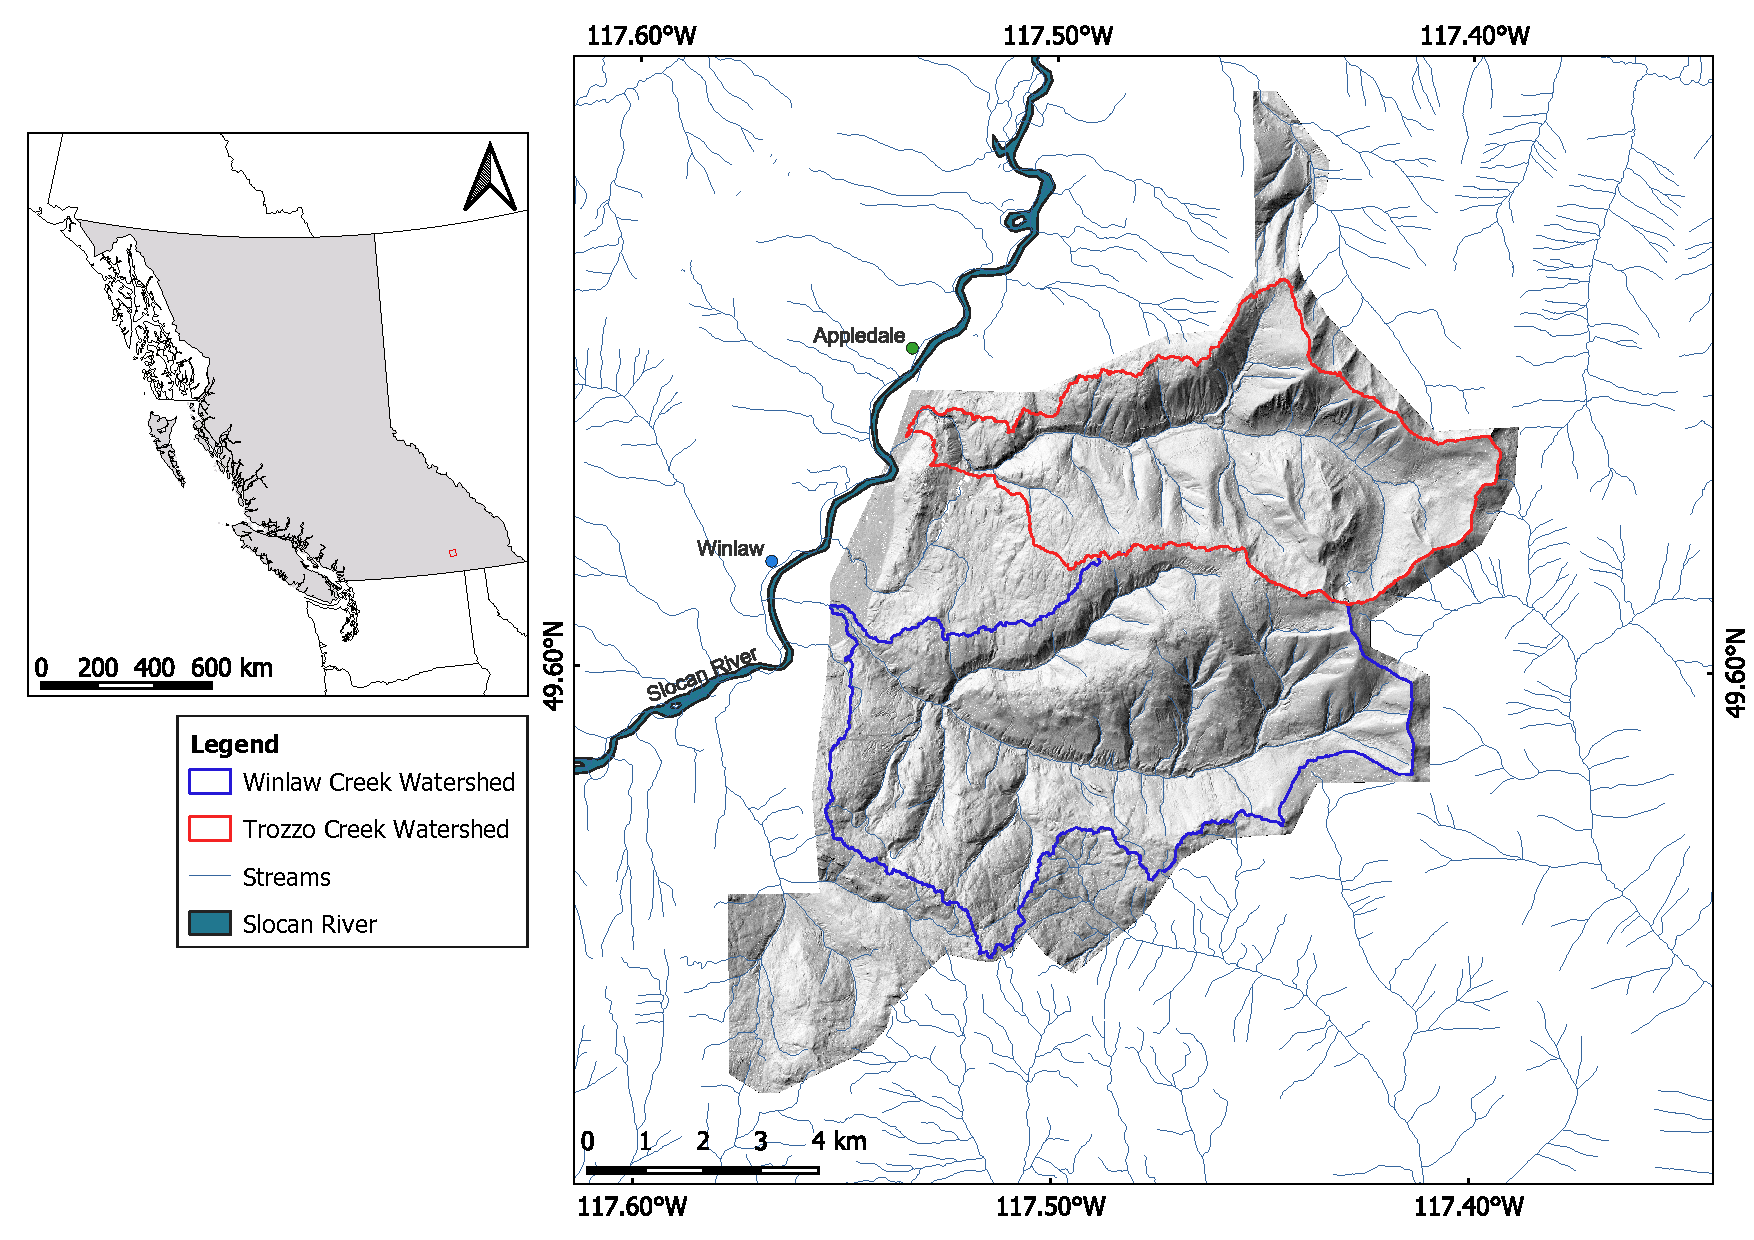
\includegraphics[width=1\textwidth,height=\textheight]{img/studyarea.png}

\textbf{Figure 1} The Study area in the West Kootenay region of southeastern British Columbia, showing the two watersheds in the study area: Winlaw watershed (\textasciitilde41km\^{}2), and the Trozzo Creek Watershed (\textasciitilde28km\^{}2). Streams in the study area are shown in blue and the inset map situates the study area in the province of British Columbia.

\hypertarget{sec-required-r-packages}{%
\subsection*{RStudio Preparation:}\label{sec-required-r-packages}}
\addcontentsline{toc}{subsection}{RStudio Preparation:}

\hypertarget{packages}{%
\subsubsection*{Required R Packages:}\label{packages}}
\addcontentsline{toc}{subsubsection}{Required R Packages:}

The method for applying the RUSLE is entirely open source and is integrated within the geospatial R ecosystem (i.e.~\texttt{raster/terra/stars\ and\ sp/sf)}. This guide has been written to help both the RUSLE novice, as well as the seasoned geospatial analyst. Key packages used in this demonstration are:

\begin{Shaded}
\begin{Highlighting}[]
\FunctionTok{library}\NormalTok{(magrittr)}
\FunctionTok{library}\NormalTok{(kableExtra) }
\FunctionTok{library}\NormalTok{(rgeos)}
\FunctionTok{library}\NormalTok{(raster)}
\FunctionTok{library}\NormalTok{(sf)}
\FunctionTok{library}\NormalTok{(whitebox)}
\FunctionTok{library}\NormalTok{(sp)}
\FunctionTok{library}\NormalTok{(leaflet)}
\FunctionTok{library}\NormalTok{(magrittr)}
\FunctionTok{library}\NormalTok{(kableExtra)}
\FunctionTok{library}\NormalTok{(readxl)}
\end{Highlighting}
\end{Shaded}

\hypertarget{sec-rstudio-preparation}{%
\subsubsection*{Setting the Coordinate Reference System:}\label{sec-rstudio-preparation}}
\addcontentsline{toc}{subsubsection}{Setting the Coordinate Reference System:}

All input raster and vector surfaces must have the same Coordinate Reference System (CRS):

\begin{Shaded}
\begin{Highlighting}[]
\NormalTok{projection }\OtherTok{\textless{}{-}} \FunctionTok{crs}\NormalTok{(}\StringTok{"+proj=utm +zone=11 +ellps=GRS80 +units=m +no\_defs"}\NormalTok{)}
\end{Highlighting}
\end{Shaded}

\hypertarget{sec-factor-1-method}{%
\subsection*{Factor 1 - Rainfall Erosivity (R)}\label{sec-factor-1-method}}
\addcontentsline{toc}{subsection}{Factor 1 - Rainfall Erosivity (R)}

\hypertarget{sec-R-input-data}{%
\subsubsection*{Input Data:}\label{sec-R-input-data}}
\addcontentsline{toc}{subsubsection}{Input Data:}

Data for the R factor is sourced from the \href{https://esdac.jrc.ec.europa.eu/content/global-rainfall-erosivity\#tabs-0-description=1}{Rainfall erosivity dataset (2017)}. The provided R-factor map at resolutions of 30 arc-sec (\textasciitilde1 km at the Equator). This data offers complete global rainfall erosivity data based on 3625 precipitation stations and around 60,000 years of rainfall records at high temporal resolution (1 to 60 minutes). Rainfall erosivity values (MJ mm ha-1 h-1 yr-1) for the study area range between 483.7963 and 622.4443 MJ mm ha-1 h-1 yr-1. These values are consistent with those reported for British Columbia. For example, according to a report by \href{https://sis.agr.gc.ca/cansis/publications/manuals/2002-92/rusle-can.pdf}{Agriculture and Agri-Food Canada}, R values in Vancouver, B.C. are approximately 378 MJ mm ha-1 h-1. Marginally lower R values in the study area are explained by the geographic location of the study area, being inland from the west coast temperate zone.

\hypertarget{sec-calculating-the-r-factor}{%
\subsubsection*{Calculating the R Factor:}\label{sec-calculating-the-r-factor}}
\addcontentsline{toc}{subsubsection}{Calculating the R Factor:}

For application with the RUSLE, the \href{https://esdac.jrc.ec.europa.eu/content/global-rainfall-erosivity\#tabs-0-description=1}{Rainfall erosivity dataset (2017)} is clipped to the study area and saved to file (\textbf{Figure 2}):

\begin{Shaded}
\begin{Highlighting}[]
\NormalTok{R\_factor }\OtherTok{\textless{}{-}} \FunctionTok{raster}\NormalTok{(}\StringTok{"data/4/R/R\_factor.tif"}\NormalTok{,  }\AttributeTok{res =} \DecValTok{1}\NormalTok{)}
\NormalTok{R\_factor }\OtherTok{\textless{}{-}} \FunctionTok{crop}\NormalTok{(R\_factor, crop\_extent)}
\end{Highlighting}
\end{Shaded}

\includegraphics[width=1\textwidth,height=\textheight]{img/r_factor.png}

\textbf{Figure 2}: Rainfall factor (R) values, measured in MJ mm ha-1 h-1 yr-1, for the Winlaw and Trozzo Creek watersheds. The highest R values (max = 622) in the study area are located in the southwest, and the lowest values (min = 484) are located in the northeast. Data sourced from the \href{https://esdac.jrc.ec.europa.eu/content/global-rainfall-erosivity\#tabs-0-description=1}{Rainfall erosivity dataset (2017)}.

\hypertarget{sec-factor-2}{%
\subsection*{Factor 2 - Slope Length (LS)}\label{sec-factor-2}}
\addcontentsline{toc}{subsection}{Factor 2 - Slope Length (LS)}

In this study, the LS factor is calculated based \href{https://www.researchgate.net/publication/233425999_A_GIS_procedure_for_automatically_calculating_the_USLE_LS_factor_on_topographically_complex_landscape_units}{Desmet and Gover., 1996}. Following \href{https://www.researchgate.net/publication/233425999_A_GIS_procedure_for_automatically_calculating_the_USLE_LS_factor_on_topographically_complex_landscape_units}{Desmet and Gover., 1996} several sub-factors are calculated and used to inform the production of a final LS raster surface.

\hypertarget{sec-ls-input-data}{%
\subsubsection*{Input Data:}\label{sec-ls-input-data}}
\addcontentsline{toc}{subsubsection}{Input Data:}

The only required input for calculating the LS factor is a Digital elevation model (DEM). Here, we test the method using a 1m resolution DEM derived from LiDAR data (\textbf{Figure 3a}) and a 25m resolution DEM (\textbf{Figure 3b}).

\begin{Shaded}
\begin{Highlighting}[]
\NormalTok{dem }\OtherTok{\textless{}{-}} \FunctionTok{raster}\NormalTok{(}\StringTok{"DTM/dem.tif"}\NormalTok{)}
\end{Highlighting}
\end{Shaded}

\begin{figure}
\centering
\includegraphics{img/dem_1m.png}
\caption{\textbf{Figure 3a}: Digital Elevation Model (DEM) in meters (m), for the Winlaw and Trozzo Creek watersheds. The maximum elevation in the study area is 1,816 m and the minimum is 678 m. The DEM resolution is 1m.}
\end{figure}

\begin{figure}
\centering
\includegraphics{img/dem_25m.png}
\caption{\textbf{Figure 3b}: Digital Elevation Model (DEM) in meters (m), for the Winlaw and Trozzo Creek watersheds. The maximum elevation in the study area is 1,816 m and the minimum is 678 m. The DEM resolution is 25m.}
\end{figure}

\hypertarget{sec-calculating-the-ls-factor}{%
\subsubsection*{Calculating the LS Factor:}\label{sec-calculating-the-ls-factor}}
\addcontentsline{toc}{subsubsection}{Calculating the LS Factor:}

Calculating the LS factor involves nine steps:

\hypertarget{sec-step-1-ls}{%
\paragraph*{Step 1: Slope Raster}\label{sec-step-1-ls}}
\addcontentsline{toc}{paragraph}{Step 1: Slope Raster}

The first step in calumniating the LS factor is the production of twp slope raster's using the 1m DEM and 25m DEM (see \textbf{Figure 4a and 4b})).

\begin{Shaded}
\begin{Highlighting}[]
\DocumentationTok{\#\#\# Slope {-} Degrees}
\FunctionTok{wbt\_slope}\NormalTok{(}
  \AttributeTok{dem =} \StringTok{"DTM/dem.tif"}\NormalTok{, }
  \AttributeTok{output =} \StringTok{"SLOPE/slope\_degrees.tif"}\NormalTok{,}
  \AttributeTok{zfactor =} \ConstantTok{NULL}\NormalTok{, }
  \AttributeTok{units =} \StringTok{"degrees"}\NormalTok{)}
\NormalTok{slope\_degrees }\OtherTok{\textless{}{-}} \FunctionTok{raster}\NormalTok{(}\StringTok{"SLOPE/slope\_degrees.tif"}\NormalTok{)}
\end{Highlighting}
\end{Shaded}

\begin{figure}
\centering
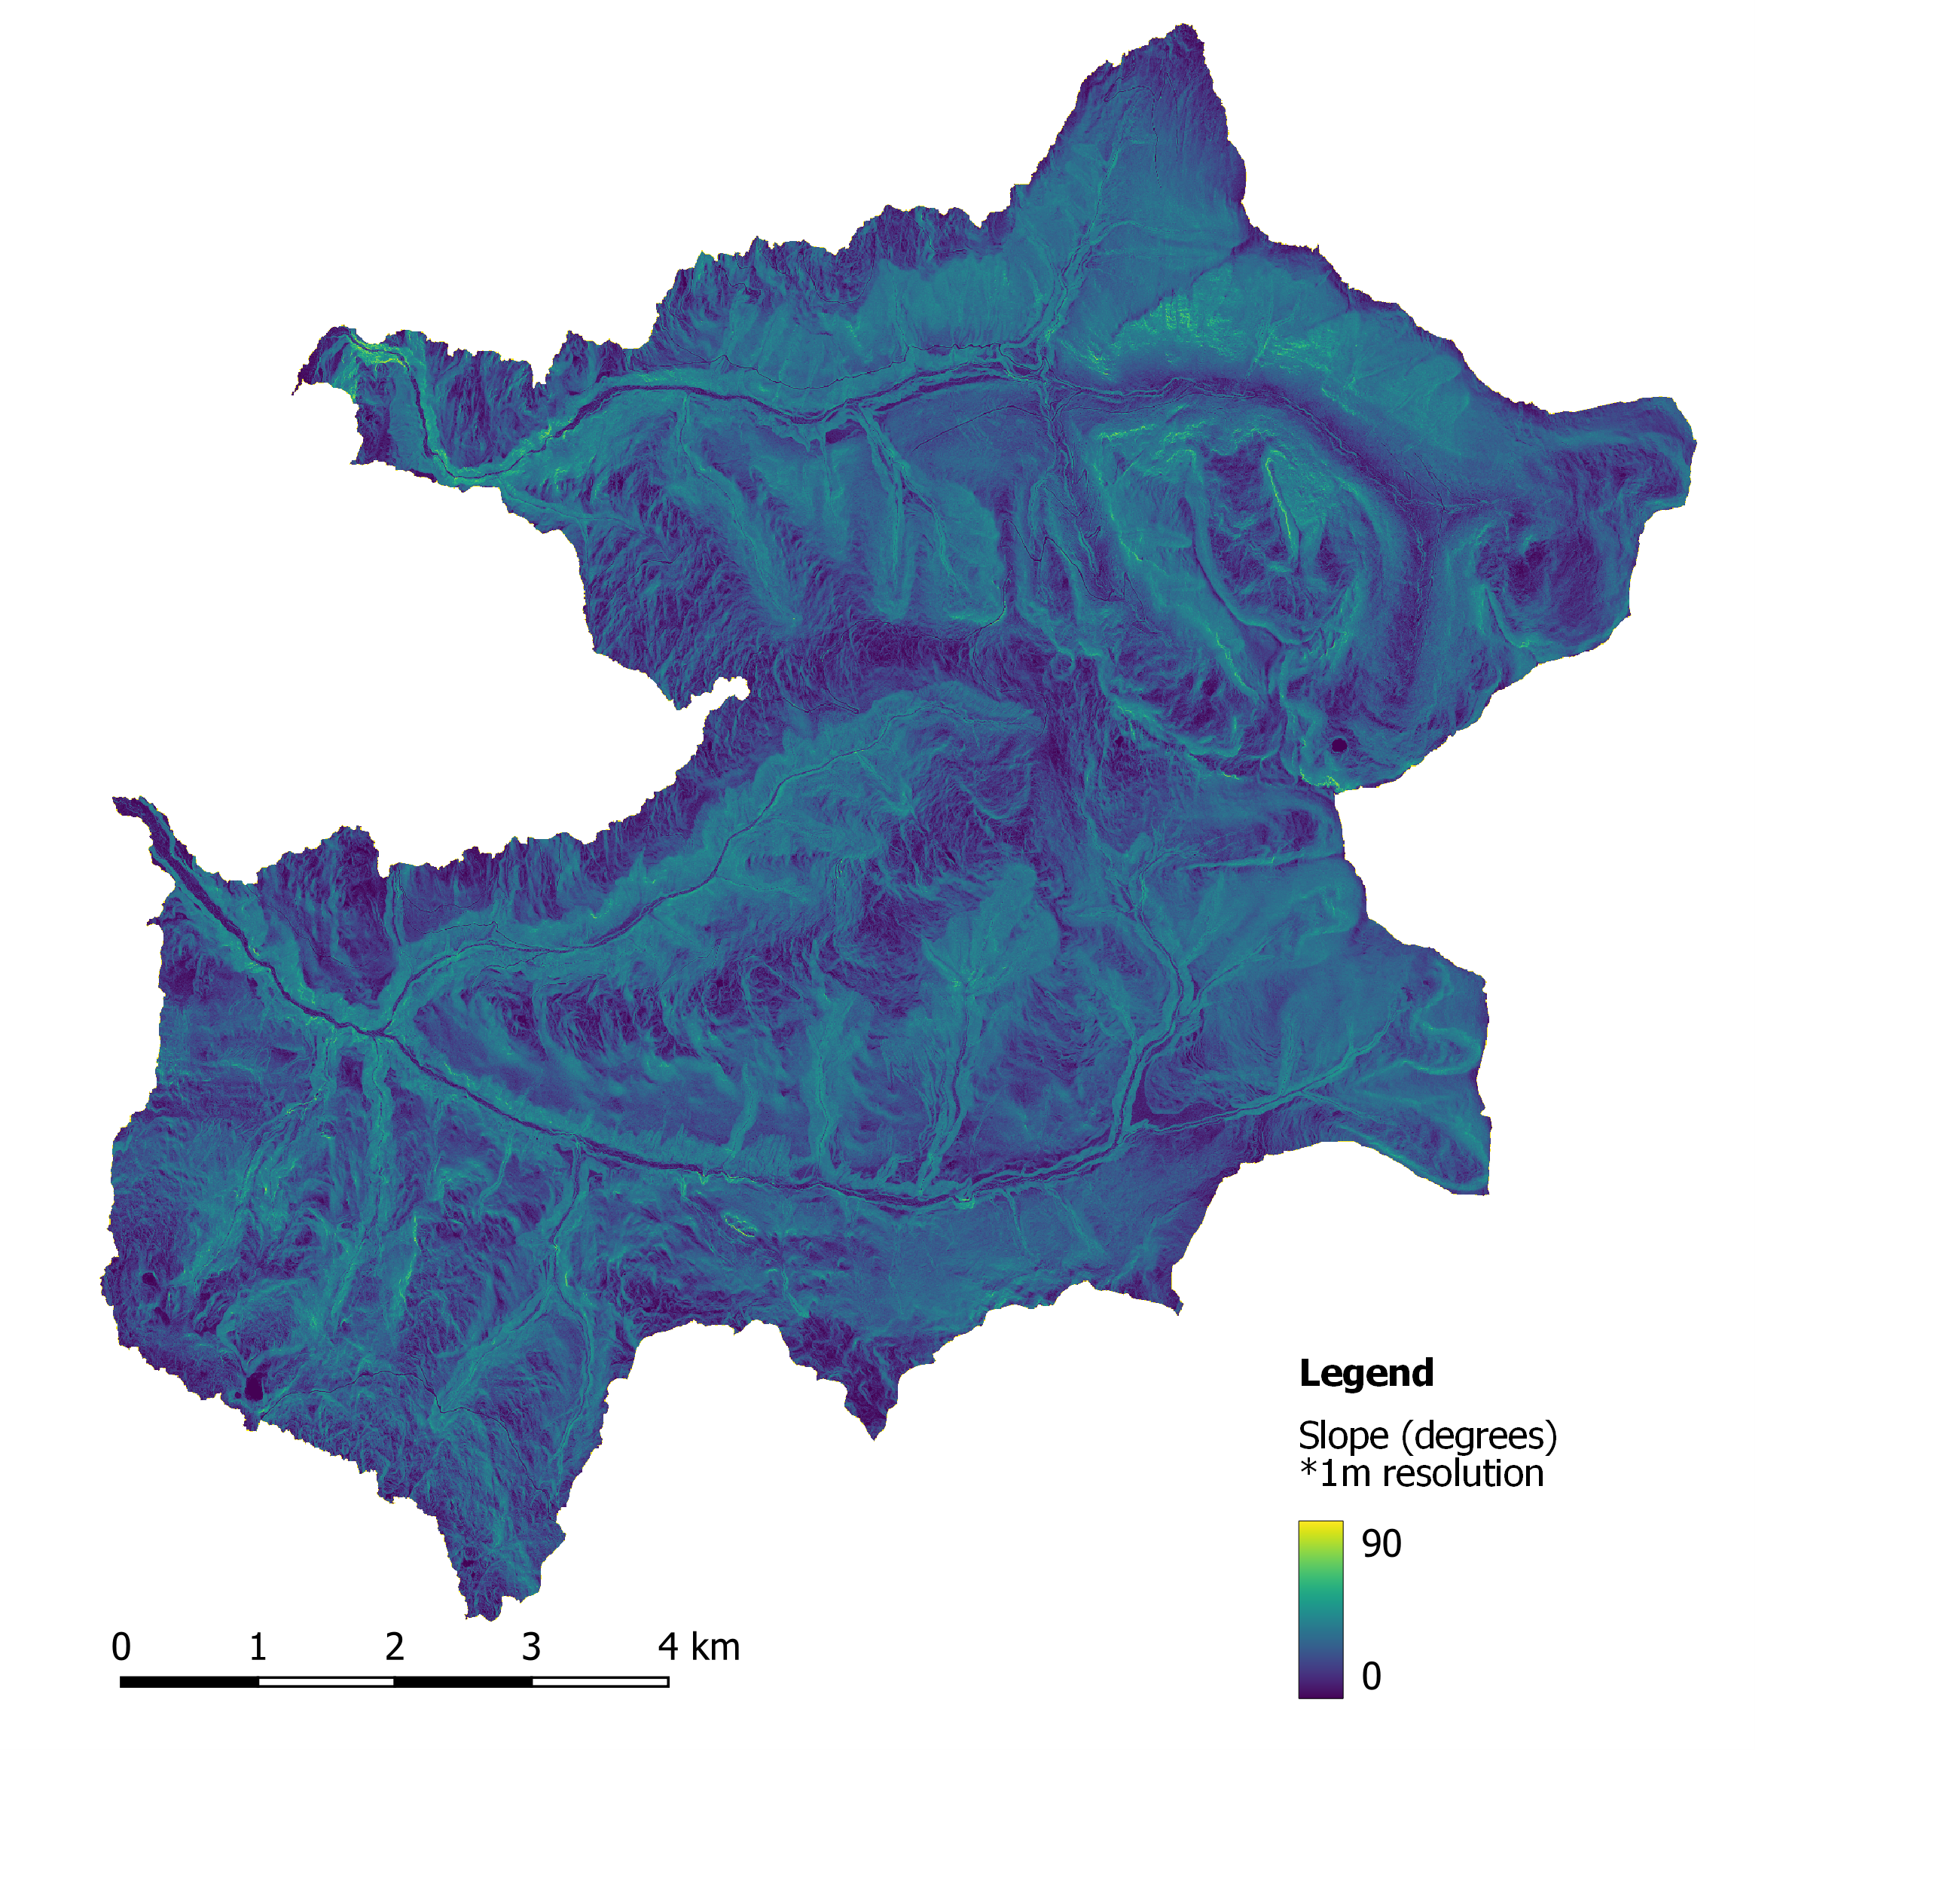
\includegraphics{img/slope_degrees_1m.png}
\caption{\textbf{Figure 4a}: Slope raster in degrees, for the Winlaw and Trozzo Creek watersheds. The maximum slope in the study area is 90 degrees and the minimum is 0 degrees. The DEM resolution is 1m.}
\end{figure}

\begin{figure}
\centering
\includegraphics{img/slope_degrees_25m.png}
\caption{\textbf{Figure 4b}: Slope raster in degrees, for the Winlaw and Trozzo Creek watersheds. The maximum slope in the study area is 90 degrees and the minimum is 0 degrees. The DEM resolution is 25m.}
\end{figure}

The slope is also produced in percent using the following code:

\begin{Shaded}
\begin{Highlighting}[]
\DocumentationTok{\#\#\# Slope {-} Percent}
\FunctionTok{wbt\_slope}\NormalTok{(}
  \AttributeTok{dem =} \StringTok{"DTM/dem.tif"}\NormalTok{, }
  \AttributeTok{output =} \StringTok{"SLOPE/slope\_percent.tif"}\NormalTok{,}
  \AttributeTok{zfactor =} \ConstantTok{NULL}\NormalTok{, }
  \AttributeTok{units =} \StringTok{"percent"}\NormalTok{)}
\NormalTok{slope\_percent }\OtherTok{\textless{}{-}} \FunctionTok{raster}\NormalTok{(}\StringTok{"SLOPE/slope\_percent.tif"}\NormalTok{)}
\end{Highlighting}
\end{Shaded}

\hypertarget{sec-step-2-ls}{%
\paragraph*{Step 2: Beta}\label{sec-step-2-ls}}
\addcontentsline{toc}{paragraph}{Step 2: Beta}

Next, Beta is calculated using the 1m and 25m resolution \texttt{slope\_degrees} rasters generated in Step 1 and the formula proposed by \href{https://www.researchgate.net/publication/233425999_A_GIS_procedure_for_automatically_calculating_the_USLE_LS_factor_on_topographically_complex_landscape_units}{Desmet and Gover., 1996} (\textbf{Figure 5a and 5b}).

\begin{Shaded}
\begin{Highlighting}[]
\NormalTok{θ }\OtherTok{\textless{}{-}}\NormalTok{ slope\_degrees}\SpecialCharTok{*}\NormalTok{pi}\SpecialCharTok{/}\DecValTok{180} \CommentTok{\# convert degrees to radians}
\NormalTok{beta }\OtherTok{=}\NormalTok{ ((}\FunctionTok{sin}\NormalTok{(θ))}\SpecialCharTok{/}\NormalTok{(}\FloatTok{0.0896}\NormalTok{))}\SpecialCharTok{/}\NormalTok{((}\FloatTok{0.56} \SpecialCharTok{+} \DecValTok{3} \SpecialCharTok{*}\NormalTok{ (}\FunctionTok{sin}\NormalTok{(θ))}\SpecialCharTok{**}\FloatTok{0.8}\NormalTok{))}
\end{Highlighting}
\end{Shaded}

\begin{figure}
\centering
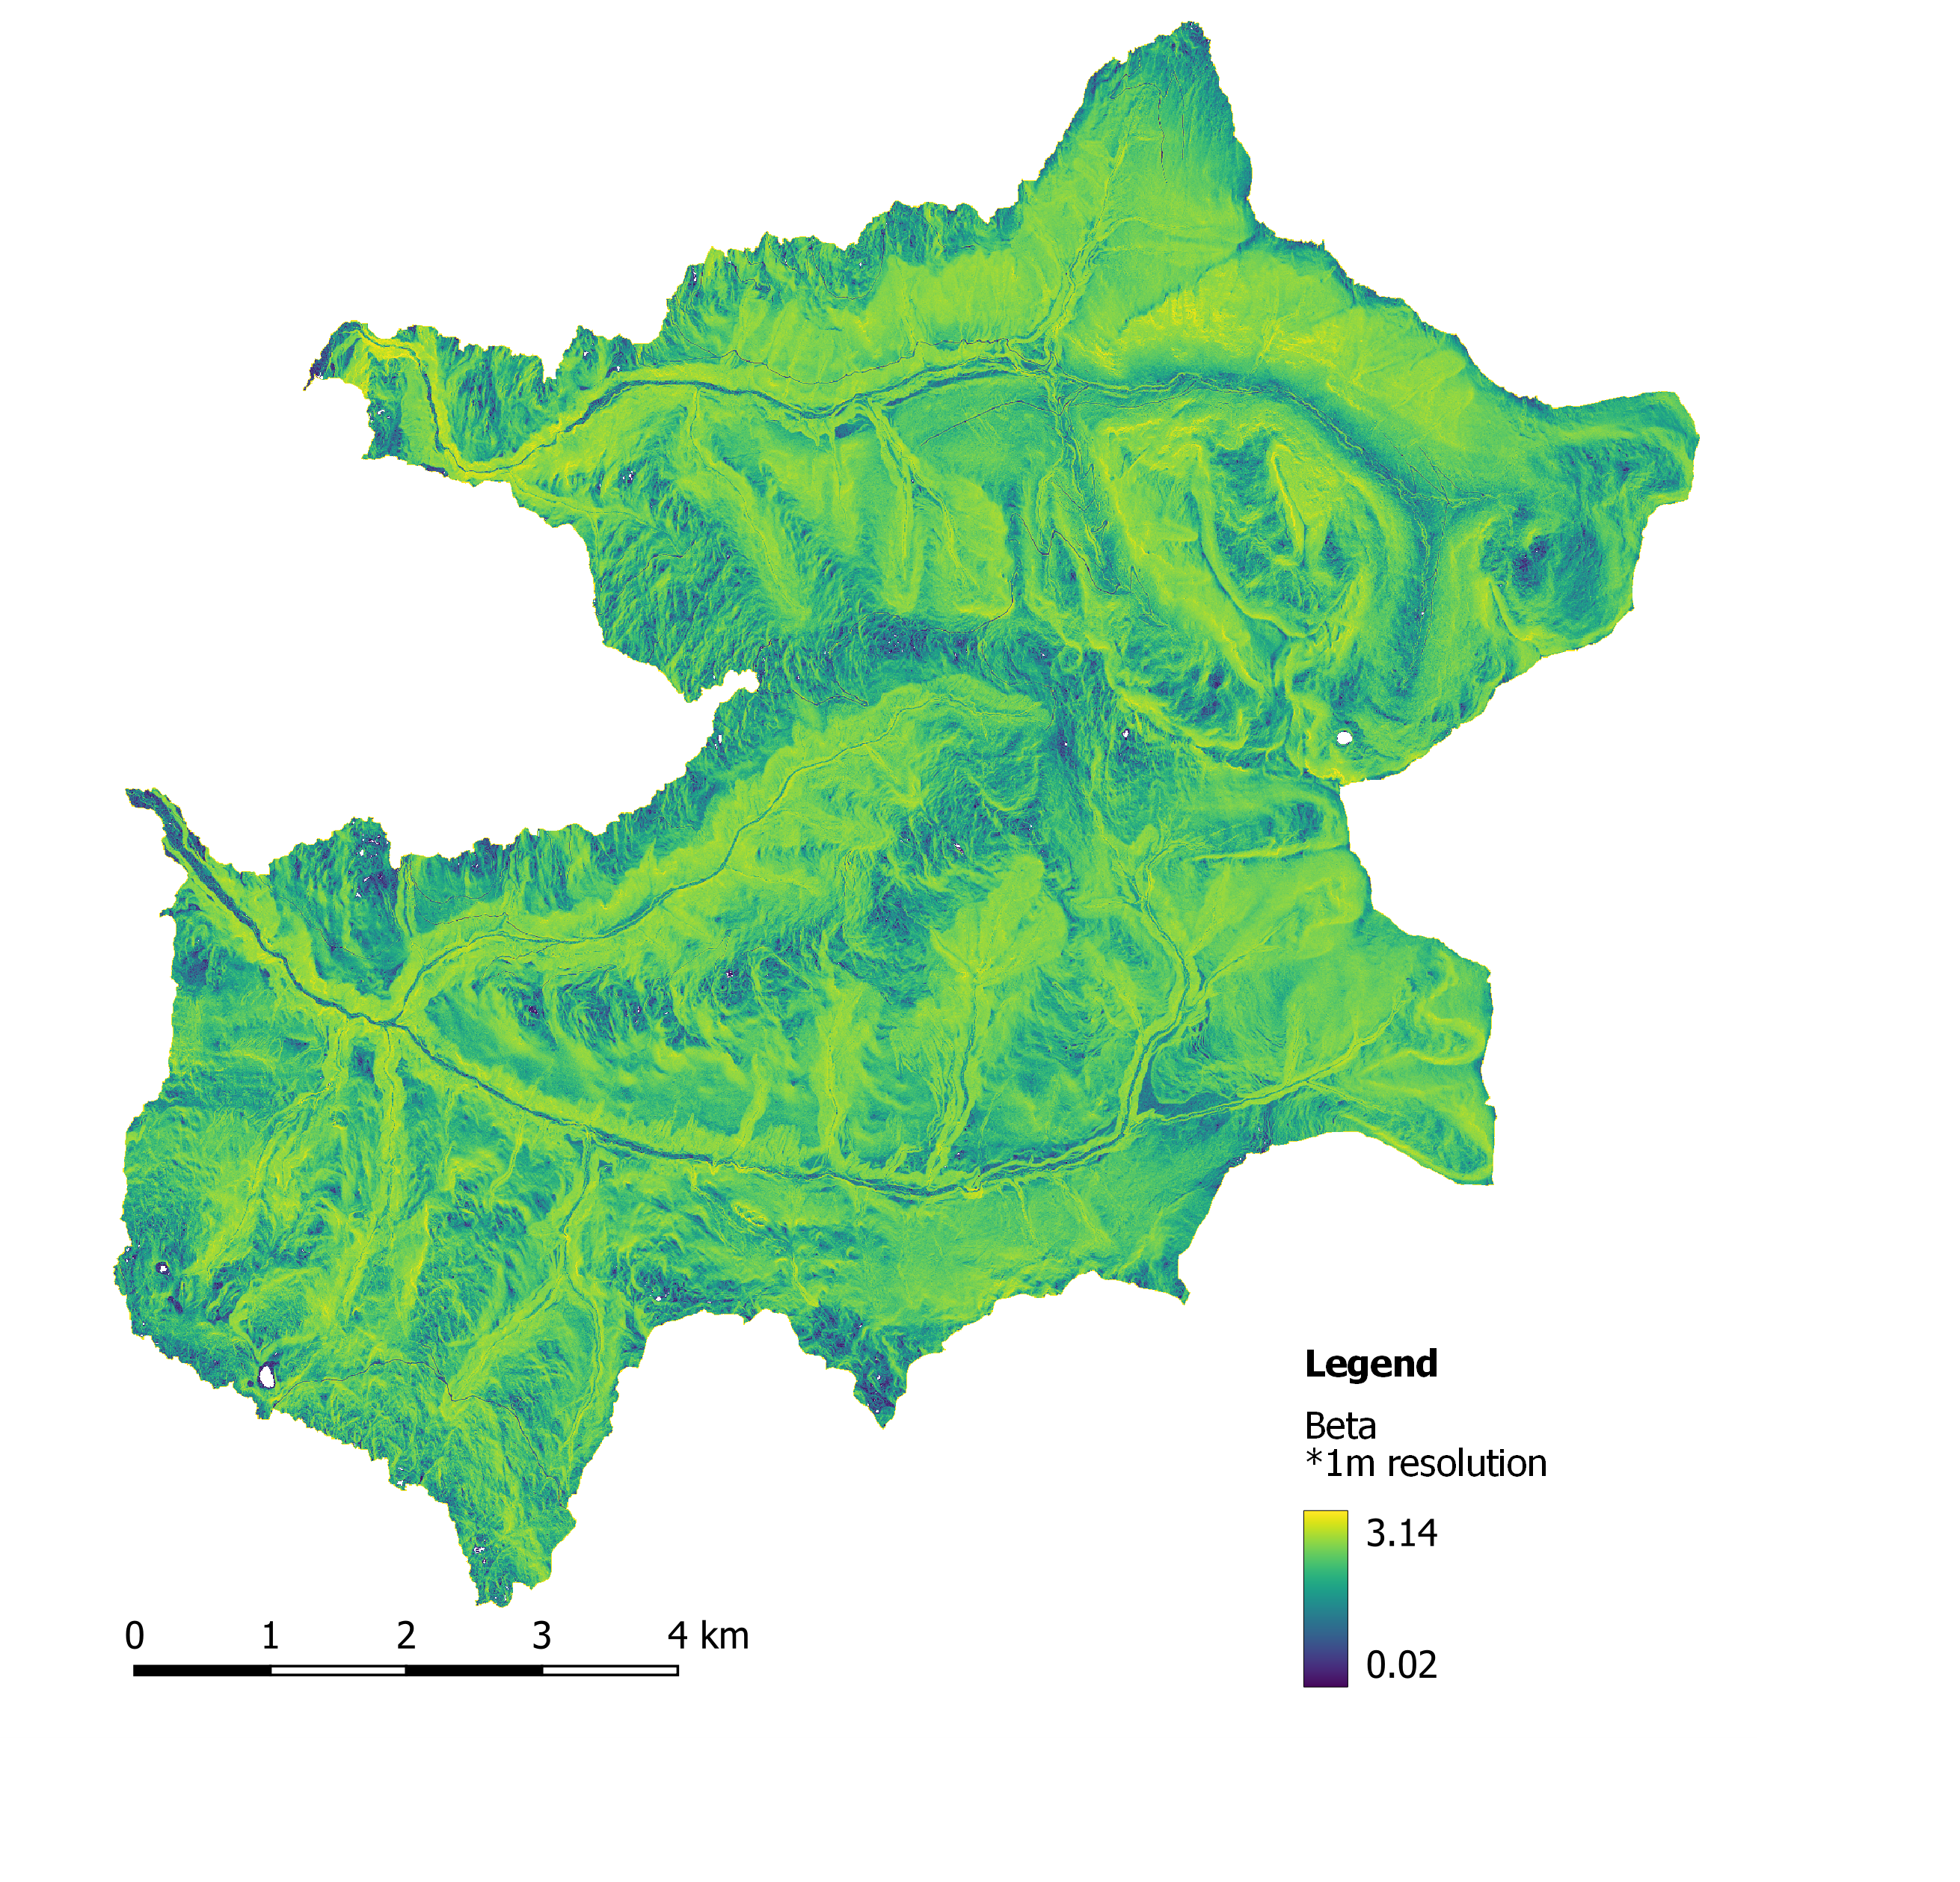
\includegraphics{img/beta_1m.png}
\caption{\textbf{Figure 5a}: Beta for the Winlaw and Trozzo Creek watersheds. The maximum value in the study area is 3.14m and the minimum value is 0.02. The beta resolution is 1m.}
\end{figure}

\begin{figure}
\centering
\includegraphics{img/beta_25m.png}
\caption{\textbf{Figure 5b}: Beta for the Winlaw and Trozzo Creek watersheds. The maximum value in the study area is 2.98m and the minimum value is 0. The beta resolution is 25m.}
\end{figure}

\hypertarget{sec-step-3-ls}{%
\paragraph*{Step 3: Ratio of Rill to Interrill Erosivity (m)}\label{sec-step-3-ls}}
\addcontentsline{toc}{paragraph}{Step 3: Ratio of Rill to Interrill Erosivity (m)}

The output of Step 2, \texttt{beta}, is used to calculate the ration of rill to interrill erosion, called \texttt{m}, for each grid cell (\textbf{Figure 6a and 6b}).

\begin{Shaded}
\begin{Highlighting}[]
\NormalTok{m }\OtherTok{=}\NormalTok{ (beta)}\SpecialCharTok{/}\NormalTok{(beta }\SpecialCharTok{+} \DecValTok{1}\NormalTok{) }\FunctionTok{plot}\NormalTok{(m)}
\end{Highlighting}
\end{Shaded}

\begin{figure}
\centering
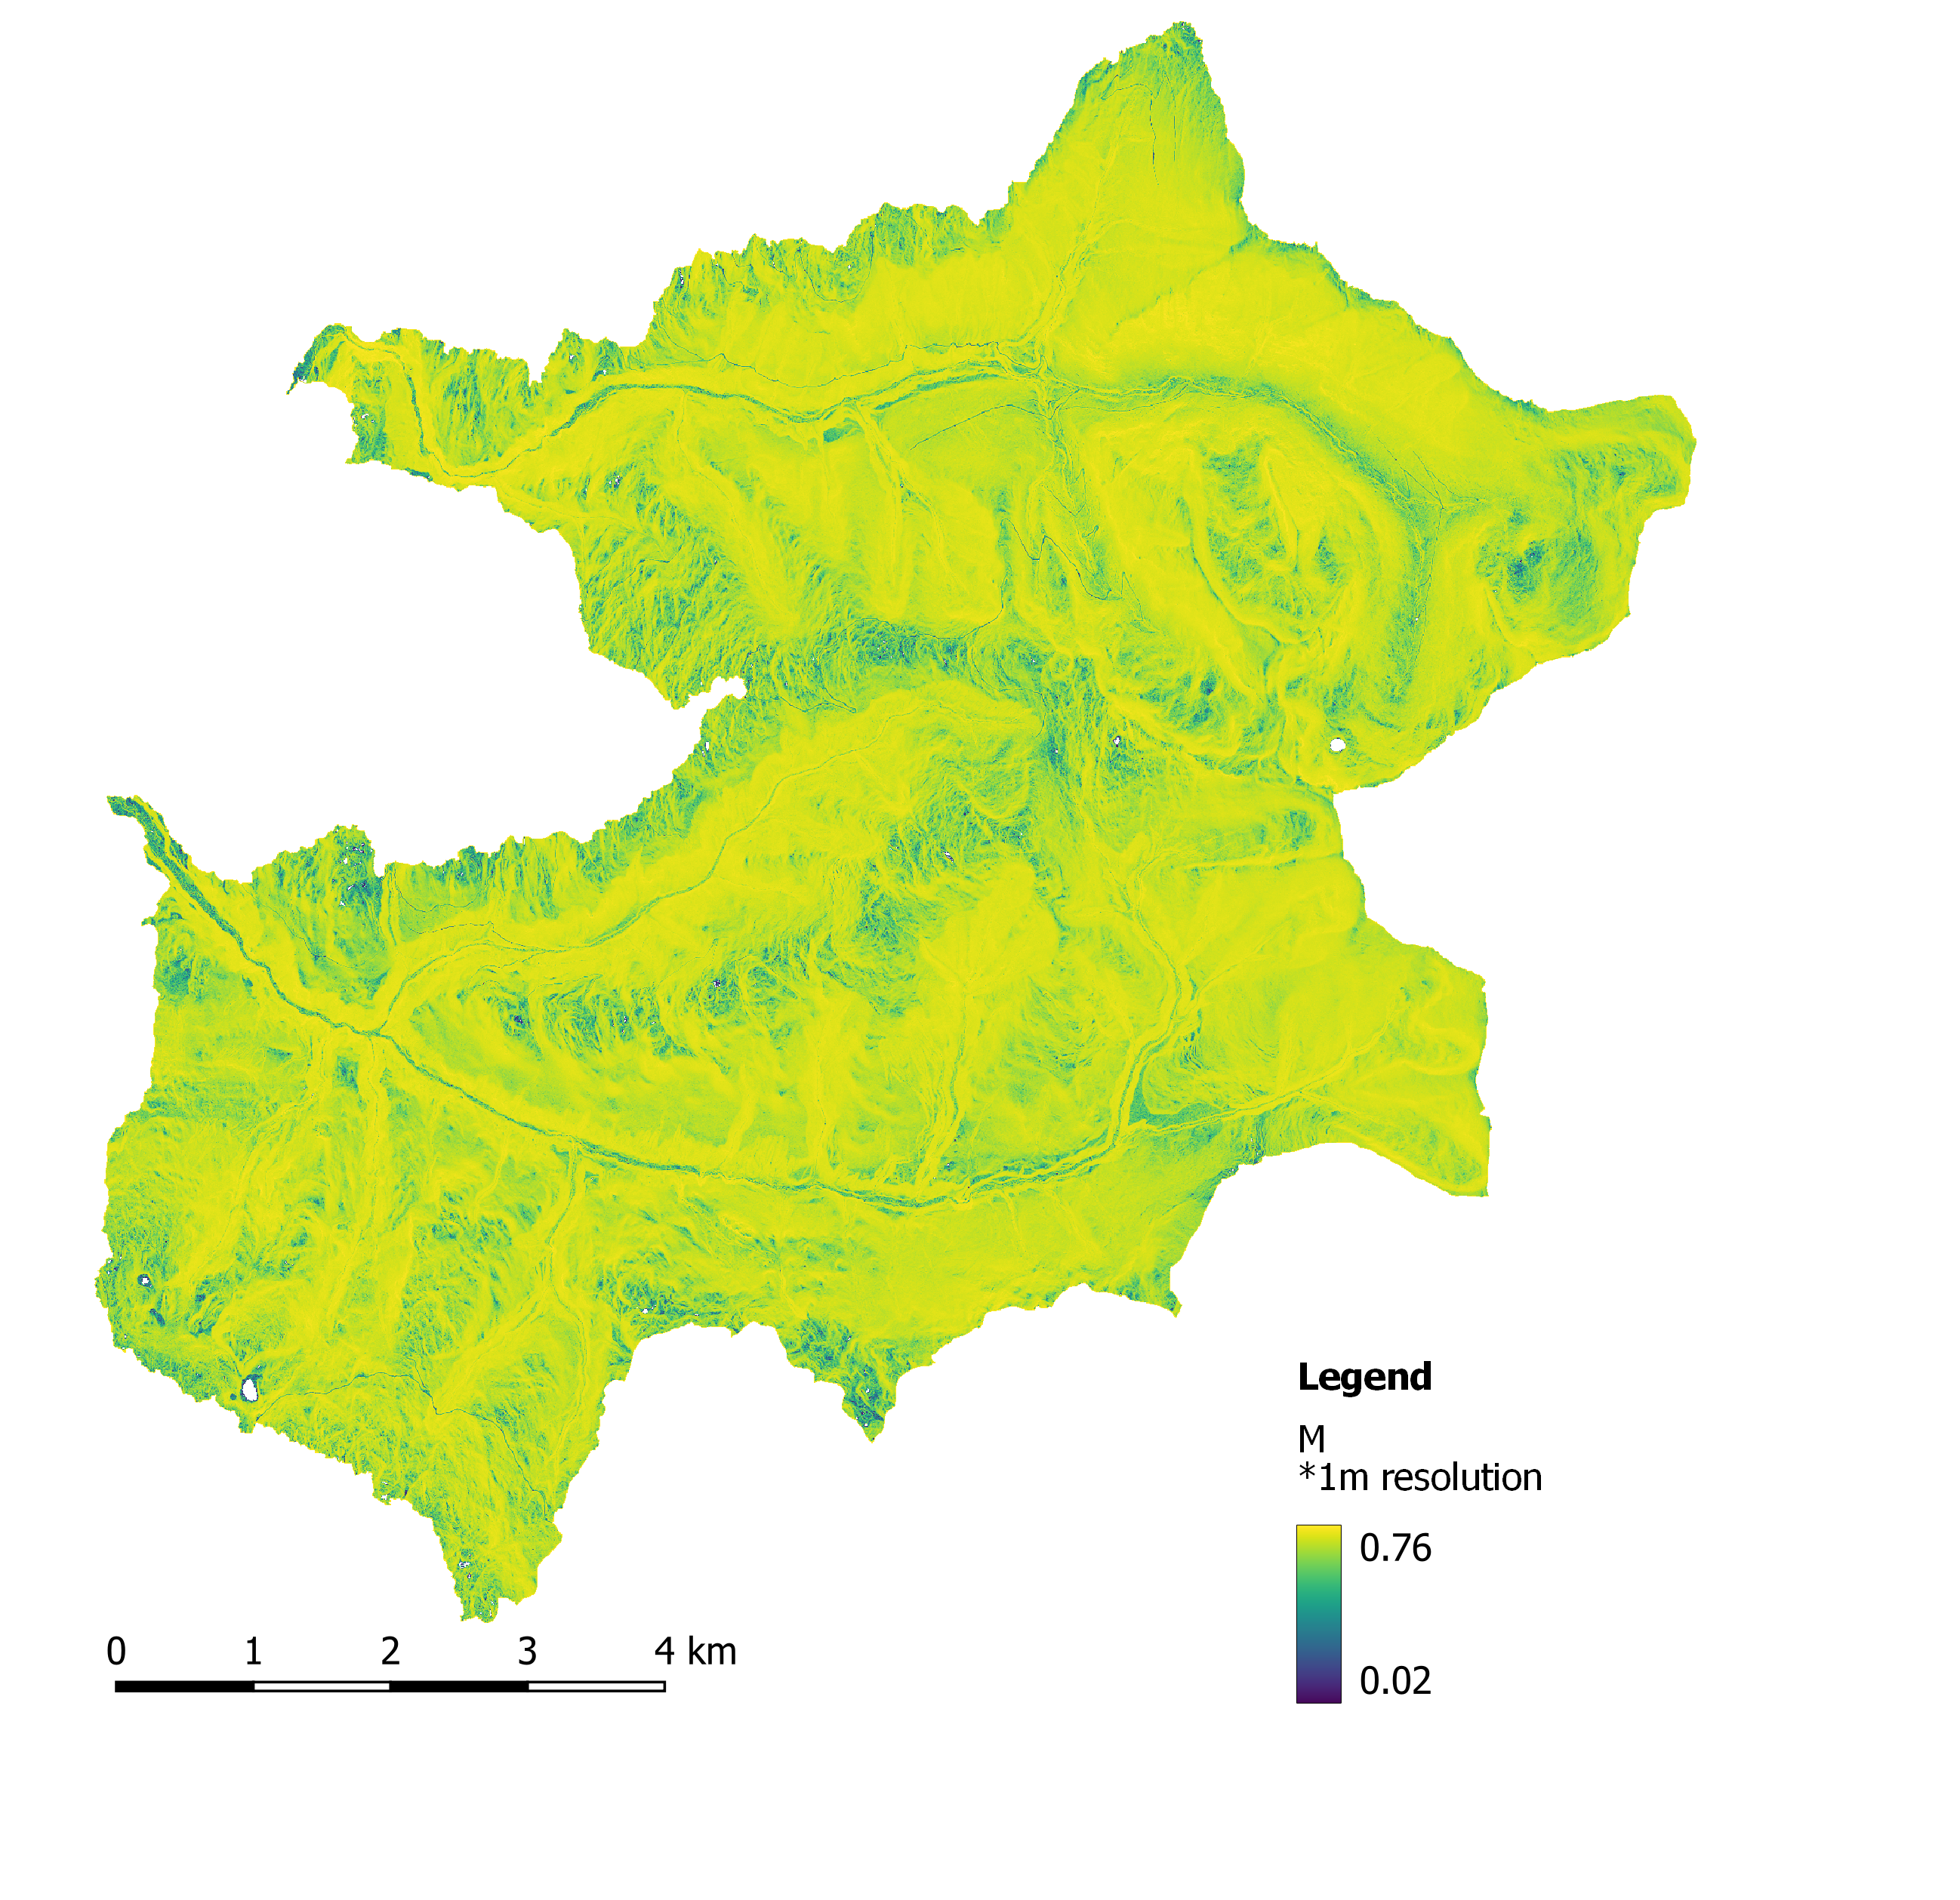
\includegraphics{img/m_1m.png}
\caption{\textbf{Figure 6a}: Ratio of Rill to Interrill Erosivity (m) for the Winlaw and Trozzo Creek watersheds. The maximum value in the study area is 0.76m and the minimum value is 0.02. The resolution is 1m.}
\end{figure}

\begin{figure}
\centering
\includegraphics{img/m_25m.png}
\caption{\textbf{Figure 6b}: Ratio of Rill to Interrill Erosivity (m) for the Winlaw and Trozzo Creek watersheds. The maximum value in the study area is 0.76m and the minimum value is 0.02. The resolution is 25m.}
\end{figure}

\hypertarget{sec-step-4-ls}{%
\paragraph*{Step 4: Aspect Raster}\label{sec-step-4-ls}}
\addcontentsline{toc}{paragraph}{Step 4: Aspect Raster}

Next, the \texttt{terrain} function from the \texttt{raster} package and the \texttt{dem} (1m and 25m) are used to produce an aspect, in radians, of the study area (\textbf{Figure 7a and 7b}).

\begin{Shaded}
\begin{Highlighting}[]
\NormalTok{aspect\_radians }\OtherTok{\textless{}{-}}  \FunctionTok{terrain}\NormalTok{(dem, }\AttributeTok{opt=}\StringTok{\textquotesingle{}aspect\textquotesingle{}}\NormalTok{, }\AttributeTok{unit=}\StringTok{\textquotesingle{}radians\textquotesingle{}}\NormalTok{, }\AttributeTok{neighbors=}\DecValTok{8}\NormalTok{, }
                           \AttributeTok{filename=} \StringTok{"ASPECT/aspect\_radians.tif"}\NormalTok{)}
\end{Highlighting}
\end{Shaded}

\begin{figure}
\centering
\includegraphics{img/aspect_1m.png}
\caption{\textbf{Figure 7a}: Aspect, in radians, for the Winlaw and Trozzo Creek watersheds. The maximum aspect value in the study area is 6.28 and the minimum value is 0 . The resolution is 1m.}
\end{figure}

\begin{figure}
\centering
\includegraphics{img/aspect_25m.png}
\caption{\textbf{Figure 7b}: Aspect, in radians, for the Winlaw and Trozzo Creek watersheds. The maximum aspect value in the study area is 6.28 and the minimum value is 0. The resolution is 25m.}
\end{figure}

\hypertarget{sec-step-5-ls}{%
\paragraph*{Step 5: Contour Width Factor (X)}\label{sec-step-5-ls}}
\addcontentsline{toc}{paragraph}{Step 5: Contour Width Factor (X)}

Using the \texttt{aspect\_radians} raster produced in Step 4 a contour width factor, named \texttt{X} , is calculated based on the method proposed by \href{https://www.researchgate.net/publication/233425999_A_GIS_procedure_for_automatically_calculating_the_USLE_LS_factor_on_topographically_complex_landscape_units}{Desmet and Gover., 1996} (\textbf{Figure 8a and 8b}).

\begin{Shaded}
\begin{Highlighting}[]
\NormalTok{sin }\OtherTok{\textless{}{-}} \FunctionTok{abs}\NormalTok{(}\FunctionTok{sin}\NormalTok{(aspect\_radians))}
\NormalTok{cos }\OtherTok{\textless{}{-}} \FunctionTok{abs}\NormalTok{(}\FunctionTok{cos}\NormalTok{(aspect\_radians))}
\NormalTok{X }\OtherTok{=} \FunctionTok{abs}\NormalTok{(}\FunctionTok{sin}\NormalTok{(aspect\_radians)) }\SpecialCharTok{+} \FunctionTok{abs}\NormalTok{(}\FunctionTok{cos}\NormalTok{(aspect\_radians))}
\end{Highlighting}
\end{Shaded}

\begin{figure}
\centering
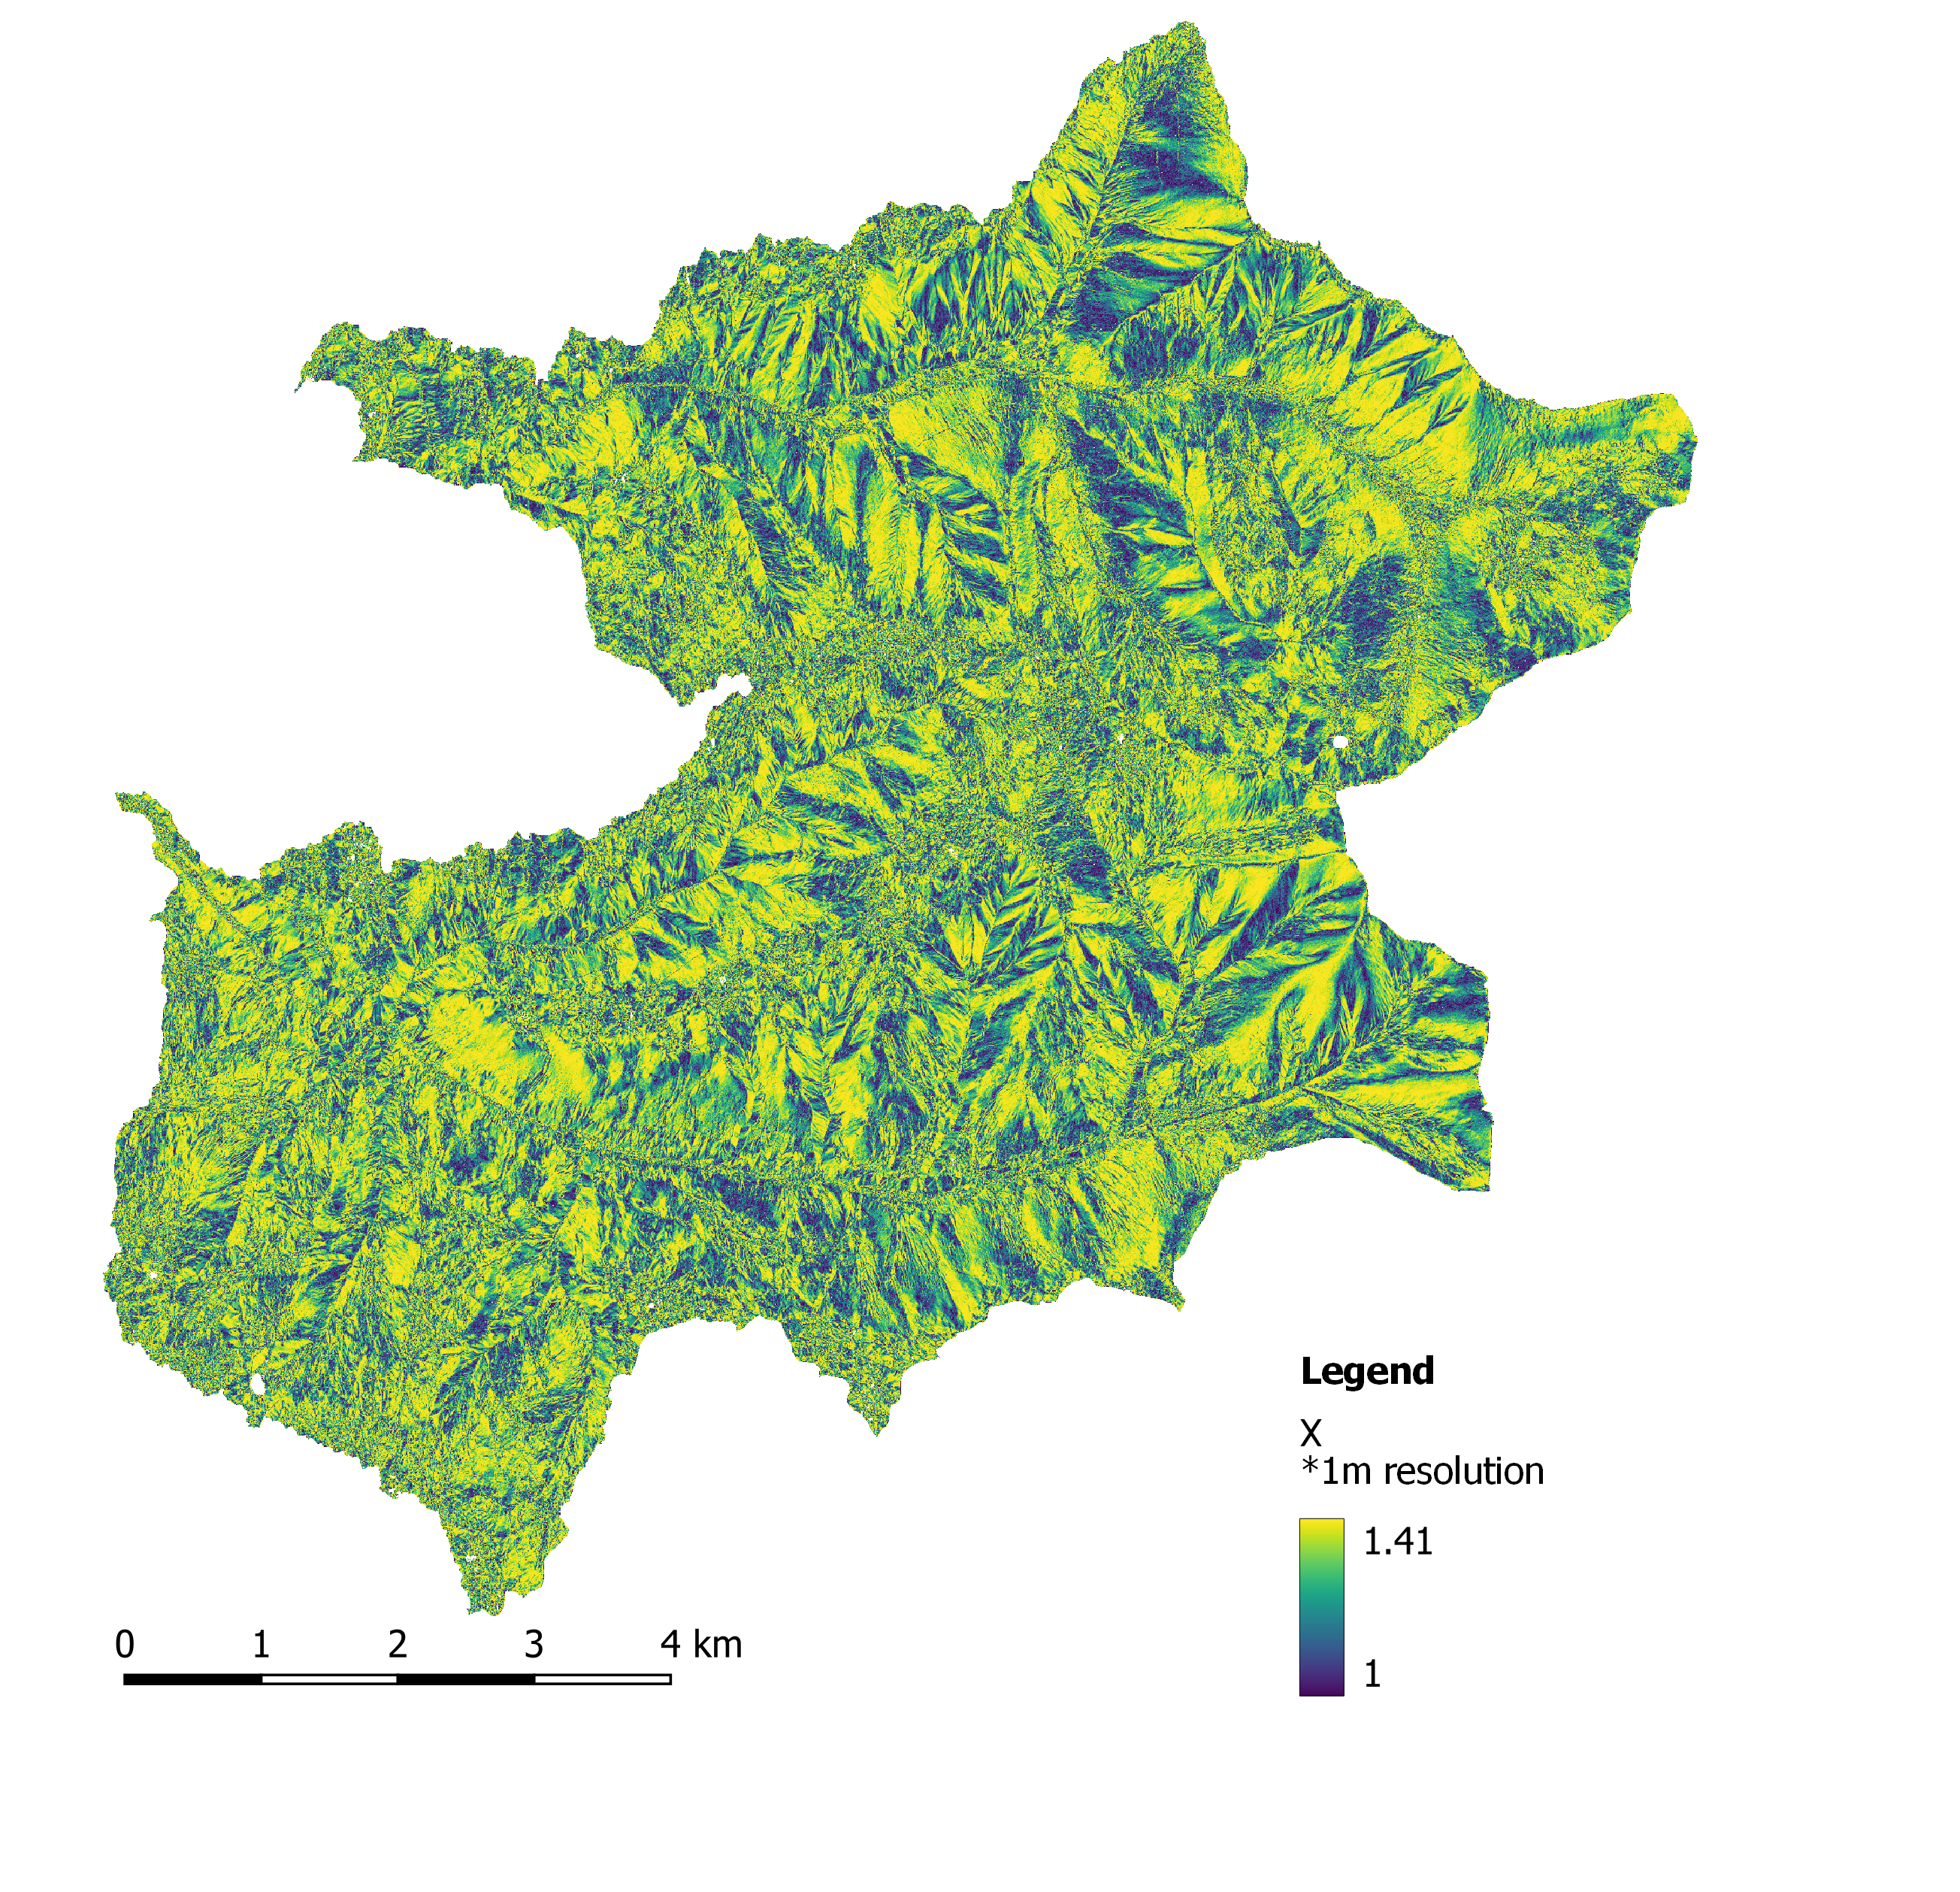
\includegraphics{img/x_1m.png}
\caption{\textbf{Figure 8a}: Contour width factor for the Winlaw and Trozzo Creek watersheds. The maximum value in the study area is 1.41 and the minimum value is 1. The resolution is 1m.}
\end{figure}

\begin{figure}
\centering
\includegraphics{img/x_25m.png}
\caption{\textbf{Figure 8b}: Contour width factor for the Winlaw and Trozzo Creek watersheds. The maximum value in the study area is 1.41 and the minimum value is 1. The resolution is 25m.}
\end{figure}

\hypertarget{sec-step-6-ls}{%
\paragraph*{Step 6: Specific Contributing Area}\label{sec-step-6-ls}}
\addcontentsline{toc}{paragraph}{Step 6: Specific Contributing Area}

Step 6 involves the production of a Specific Contributing Area raster using the \texttt{WhiteboxTools} function \texttt{wbt\_fd8\_flow\_accumulation} (\textbf{Figure 9a and 9b})).

\begin{Shaded}
\begin{Highlighting}[]
\FunctionTok{wbt\_fd8\_flow\_accumulation}\NormalTok{(}
      \AttributeTok{dem =} \StringTok{"DTM/dem.tif"}\NormalTok{, }
      \AttributeTok{output =} \StringTok{"FD8\_FLOW\_ACCUMUMULATION/fd8\_flow\_accumulation.tif"}\NormalTok{,}
      \AttributeTok{out\_type =} \StringTok{"specific contributing area"}\NormalTok{,}
      \AttributeTok{exponent =} \FloatTok{1.1}\NormalTok{,}
      \AttributeTok{log =} \ConstantTok{FALSE}
\NormalTok{    )}
\end{Highlighting}
\end{Shaded}

\begin{figure}
\centering
\includegraphics{img/a_1m_MAX.png}
\caption{\textbf{Figure 9a}: Specific contributing area (A), in pixels, for the Winlaw and Trozzo Creek watersheds. The maximum value in the study area is 358,753 pixels and the minimum value is 1 pixel. The resolution is 1m.}
\end{figure}

\begin{figure}
\centering
\includegraphics{img/fd8_1m_hist.png}
\caption{\textbf{Figure 9a (accompanying histogram):} Specific contributing area (A) for the Winlaw and Trozzo Creek watersheds. Plot showing limits set to 0 - 5000 pixels. Pixel value is 1m.}
\end{figure}

\begin{figure}
\centering
\includegraphics{img/a_25m.png}
\caption{\textbf{Figure 9b}: Specific contributing area (A) for the Winlaw and Trozzo Creek watersheds. The maximum value in the study area is 118,414 and the minimum value is 25. The resolution is 25m.}
\end{figure}

\begin{figure}
\centering
\includegraphics{img/FD8_25M_hist.png}
\caption{\textbf{Figure 9b (accompanying histogram):} Specific contributing area (A) for the Winlaw and Trozzo Creek watersheds. Plot showing limits set to 0 - 5000 pixels. Pixel value is 25m.}
\end{figure}

The Specific Contributing Area raster is edited so that all cells with a value \textgreater{} 100 are replaced with 100, our flow distance threshold. The resulting raster is named A (**Figure 10a and 10b).

\begin{Shaded}
\begin{Highlighting}[]
\NormalTok{fd8\_flow\_accumulation\_duplicate[fd8\_flow\_accumulation\_duplicate }\SpecialCharTok{\textgreater{}} \DecValTok{100}\NormalTok{] }\OtherTok{\textless{}{-}} \DecValTok{100}

\NormalTok{A }\OtherTok{\textless{}{-}}\NormalTok{ fd8\_flow\_accumulation\_duplicate}
\end{Highlighting}
\end{Shaded}

\begin{figure}
\centering
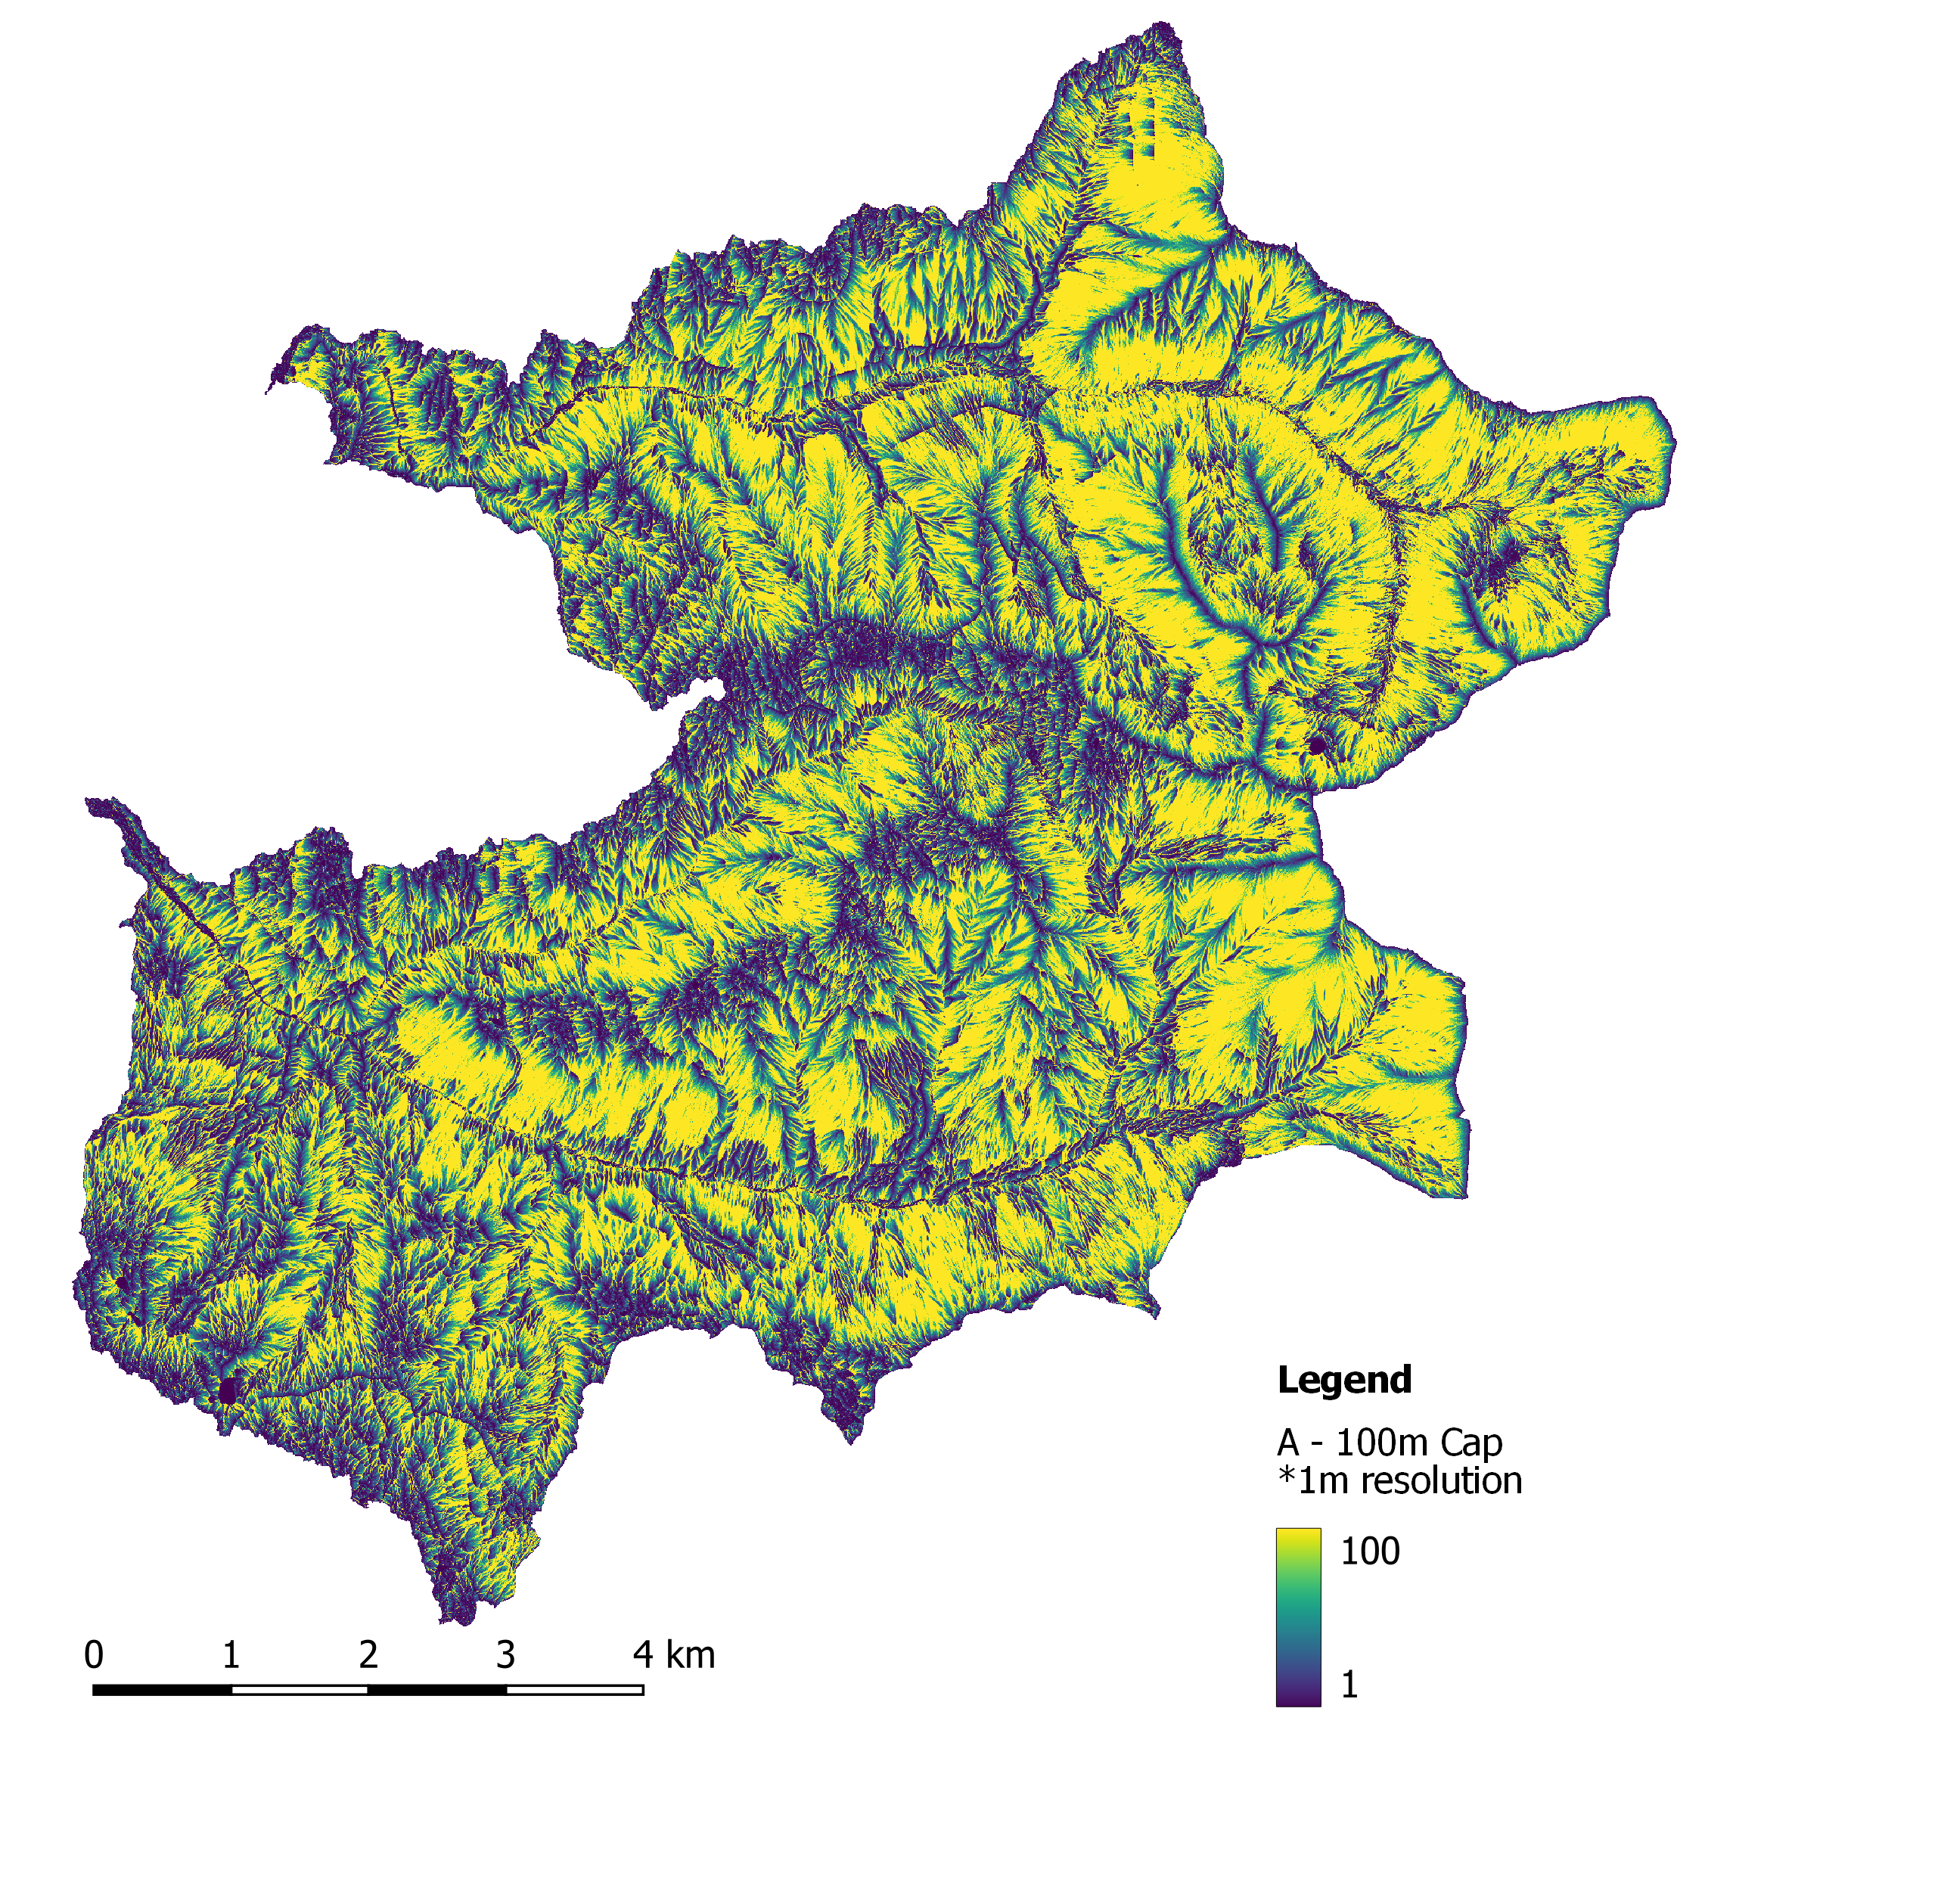
\includegraphics{img/a_1m_100m_cap.png}
\caption{\textbf{Figure 10a}: Specific contributing area (A) with a 100m threshold for the Winlaw and Trozzo Creek watersheds. The maximum value in the study area is 100 and the minimum value is 1. The resolution is 1m.}
\end{figure}

\begin{figure}
\centering
\includegraphics{img/A_1m_hist.png}
\caption{\textbf{Figure 10a (accompanying histogram)}: Specific contributing area (A) for the Winlaw and Trozzo Creek watersheds with a 100m threshold. Plot showing limits set to 0 - 100 pixels. Pixel value is 1m.}
\end{figure}

\begin{figure}
\centering
\includegraphics{img/a_25m_100m_cap.png}
\caption{\textbf{Figure 10b}: Specific contributing area (A) with a 100m threshold for the Winlaw and Trozzo Creek watersheds. The maximum value in the study area is 100 and the minimum value is 25. The resolution is 25m.}
\end{figure}

\begin{figure}
\centering
\includegraphics{img/A_25m_hist_N.png}
\caption{\textbf{Figure 10b (accompanying histogram):} Specific contributing area (A) for the Winlaw and Trozzo Creek watersheds with a 100m threshold. Plot showing limits set to 0 - 100. Pixel value is 25m.}
\end{figure}

\hypertarget{sec-step-7-ls}{%
\paragraph*{Step 7: Length (L) Raster}\label{sec-step-7-ls}}
\addcontentsline{toc}{paragraph}{Step 7: Length (L) Raster}

The length (L) component of the LS factor is calculated based on the equation proposed by \href{https://www.researchgate.net/publication/233425999_A_GIS_procedure_for_automatically_calculating_the_USLE_LS_factor_on_topographically_complex_landscape_units}{Desmet and Gover., 1996} and uses the \texttt{m,} \texttt{X}, and \texttt{A} sub-factors (\textbf{Figure 11a and 11b})).

\begin{Shaded}
\begin{Highlighting}[]
\NormalTok{L }\OtherTok{=}\NormalTok{ (((A }\SpecialCharTok{+}\NormalTok{(D}\SpecialCharTok{**}\DecValTok{2}\NormalTok{))}\SpecialCharTok{**}\NormalTok{(m}\SpecialCharTok{+}\DecValTok{1}\NormalTok{))}\SpecialCharTok{{-}}\NormalTok{(A}\SpecialCharTok{**}\NormalTok{(m}\SpecialCharTok{+}\DecValTok{1}\NormalTok{)))}\SpecialCharTok{/}\NormalTok{((D}\SpecialCharTok{**}\NormalTok{(m}\SpecialCharTok{+}\DecValTok{2}\NormalTok{))}\SpecialCharTok{*}\NormalTok{(x}\SpecialCharTok{**}\NormalTok{m)}\SpecialCharTok{*}\NormalTok{(}\FloatTok{22.13}\SpecialCharTok{**}\NormalTok{m))}
\end{Highlighting}
\end{Shaded}

\begin{figure}
\centering
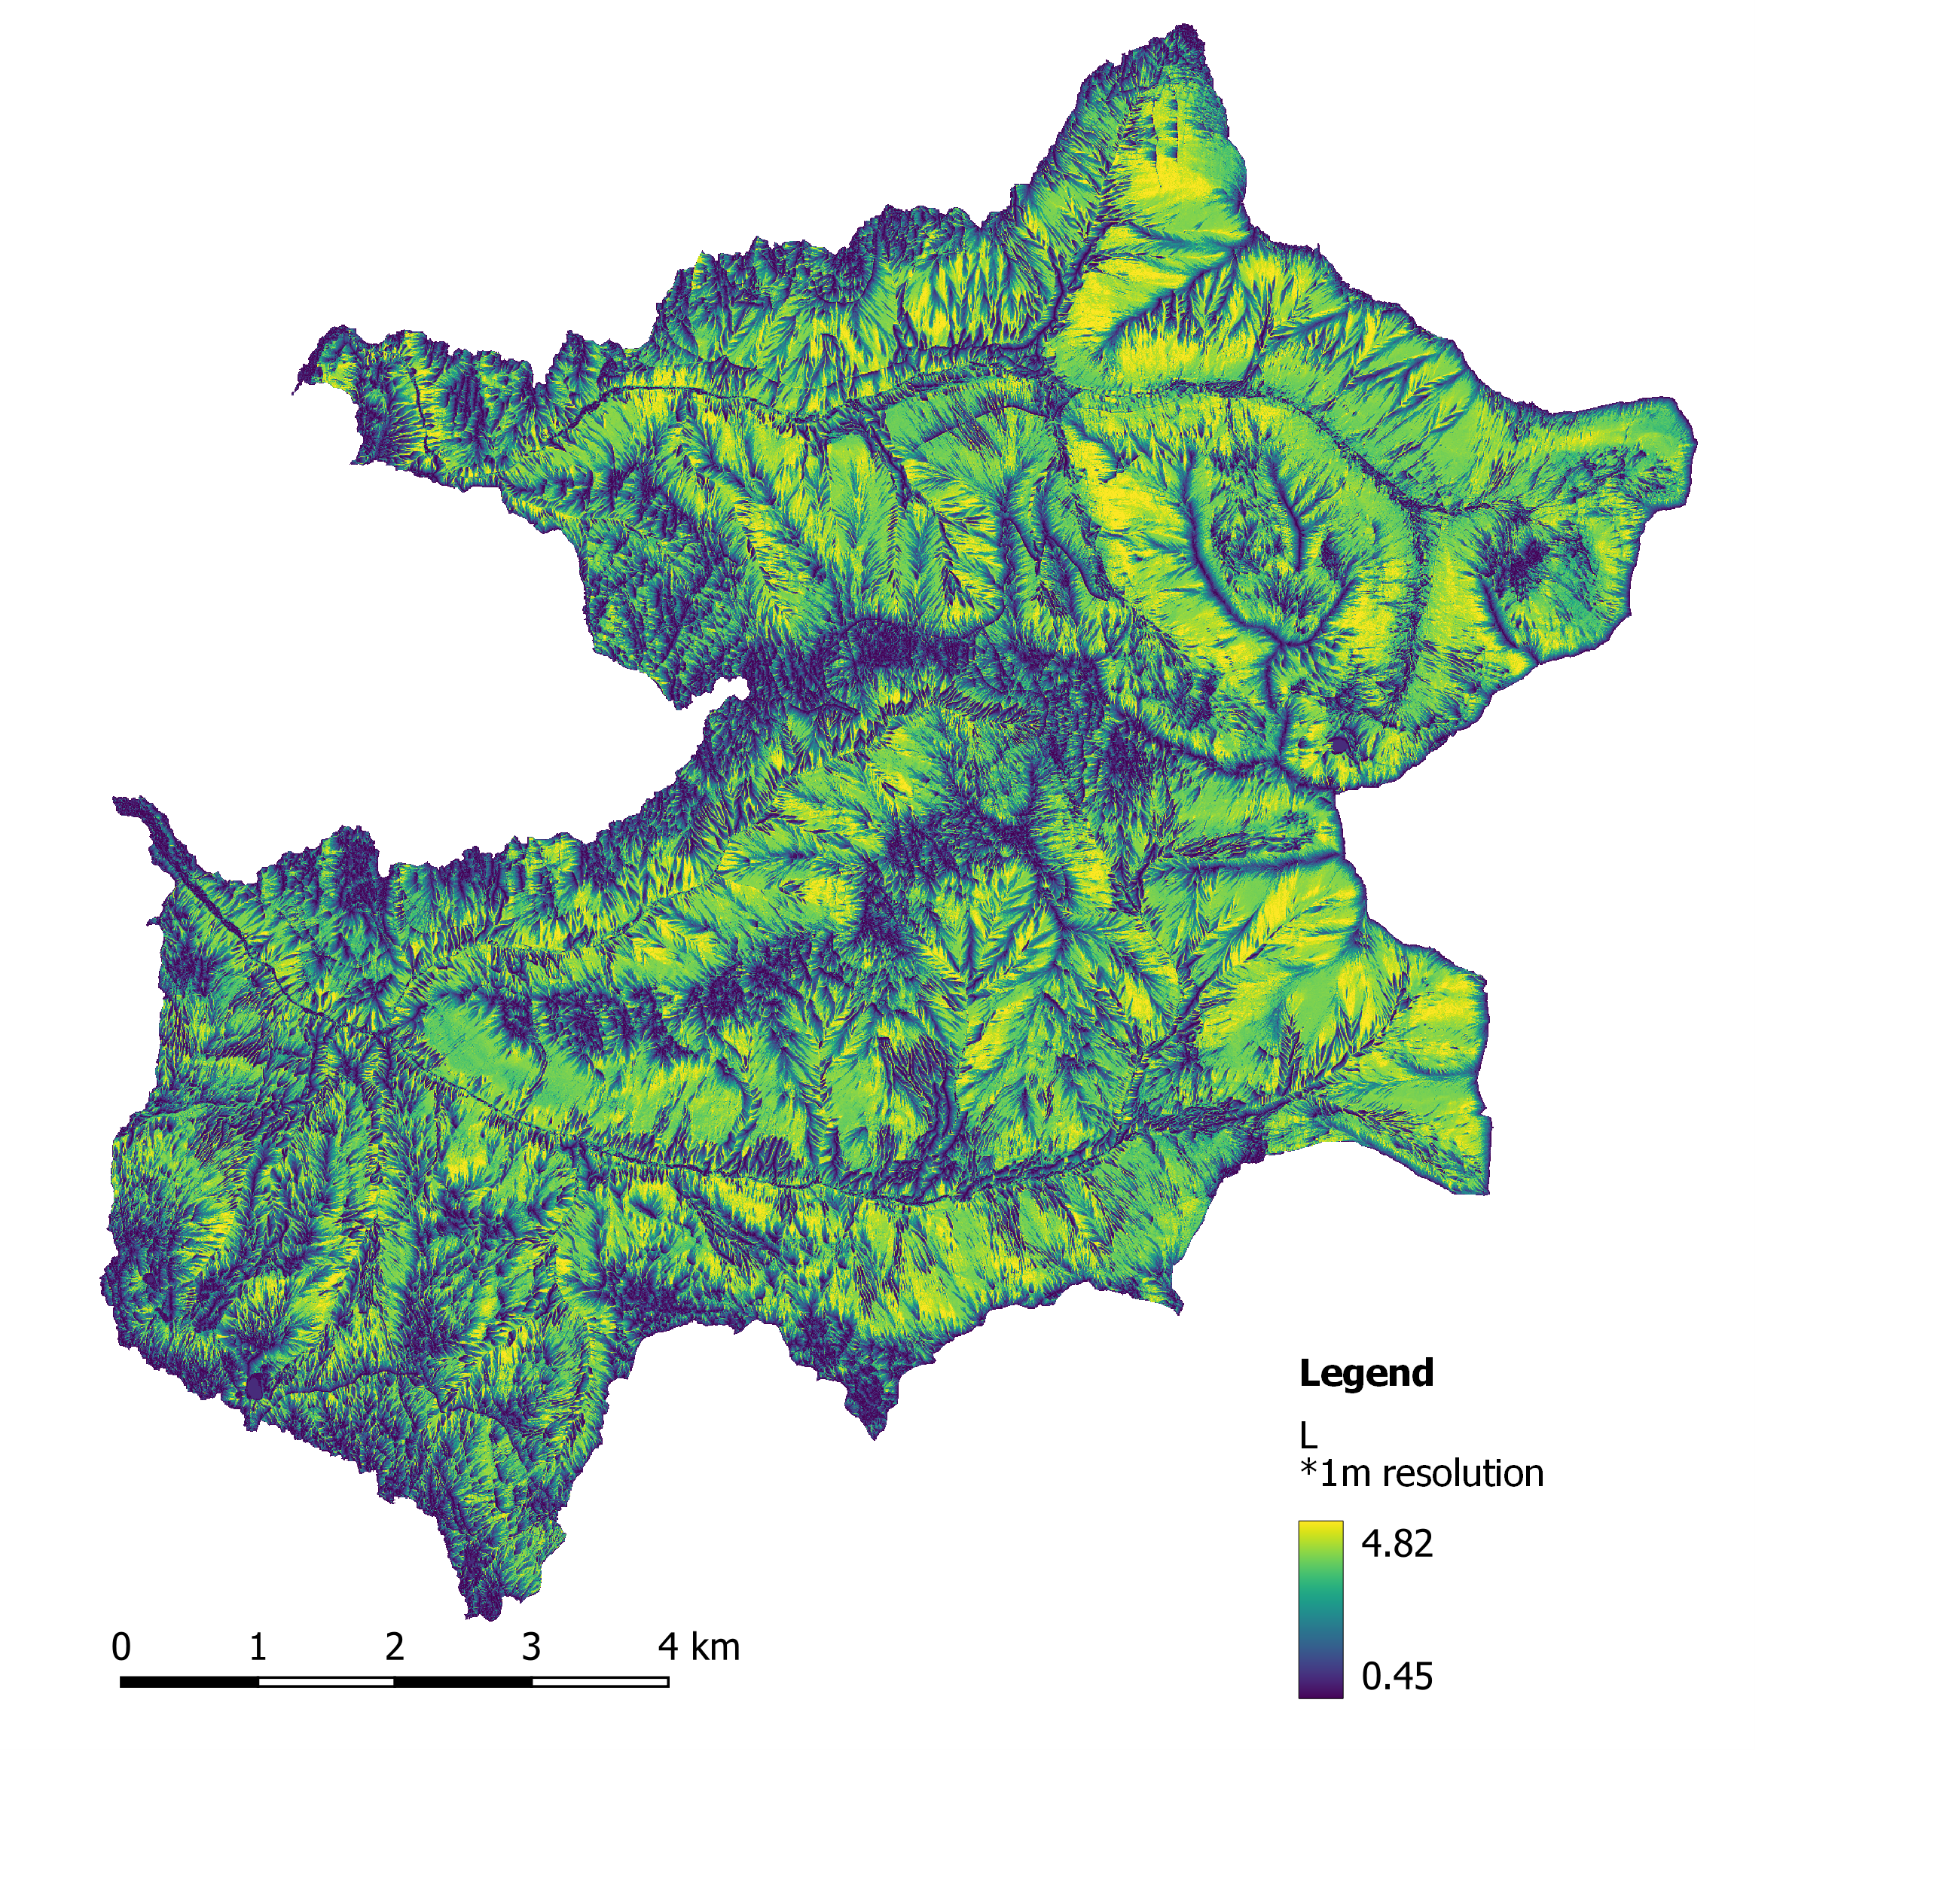
\includegraphics{img/l_1m.png}
\caption{\textbf{Figure 11a}: Length (L) factor for the Winlaw and Trozzo Creek watersheds. The maximum value in the study area is 4.82 and the minimum value is 0.45. The resolution is 1m.}
\end{figure}

\begin{figure}
\centering
\includegraphics{img/L_1m_hist.png}
\caption{\textbf{Figure 11a (accompanying histogram):} Length factor (L) for the Winlaw and Trozzo Creek watersheds. Pixel value is 1m.}
\end{figure}

\begin{figure}
\centering
\includegraphics{img/l_25m.png}
\caption{\textbf{Figure 11b}: Length (L) factor for the Winlaw and Trozzo Creek watersheds. The maximum value in the study area is 1.1 and the minimum value is 0.85. The resolution is 25m.}
\end{figure}

\begin{figure}
\centering
\includegraphics{img/L_25m_hist.png}
\caption{\textbf{Figure 11a (accompanying histogram):} Length factor (L) for the Winlaw and Trozzo Creek watersheds. Pixel value is 25m.}
\end{figure}

\hypertarget{sec-step-8-ls}{%
\paragraph*{Step 8: Slope (S) Raster}\label{sec-step-8-ls}}
\addcontentsline{toc}{paragraph}{Step 8: Slope (S) Raster}

The slope (S) component of the LS factor is calculated based on the equation proposed by \href{https://www.tandfonline.com/doi/full/10.1080/17445647.2019.1585980}{Schmidt et al.~2019} and uses the \texttt{slope\_percent} raster produced in Step 1 (\textbf{Figure 12a and 12b}).

\begin{Shaded}
\begin{Highlighting}[]
\NormalTok{S }\OtherTok{=}\NormalTok{ (}\FloatTok{0.0005}\SpecialCharTok{*}\NormalTok{(slope\_percent}\SpecialCharTok{**}\DecValTok{2}\NormalTok{)) }\SpecialCharTok{+}\NormalTok{ (}\FloatTok{0.1795}\SpecialCharTok{*}\NormalTok{slope\_percent) }\SpecialCharTok{{-}}\NormalTok{ (}\FloatTok{0.4418}\NormalTok{)}
\NormalTok{S[S }\SpecialCharTok{\textless{}} \DecValTok{0}\NormalTok{] }\OtherTok{\textless{}{-}} \DecValTok{0}
\end{Highlighting}
\end{Shaded}

\begin{figure}
\centering
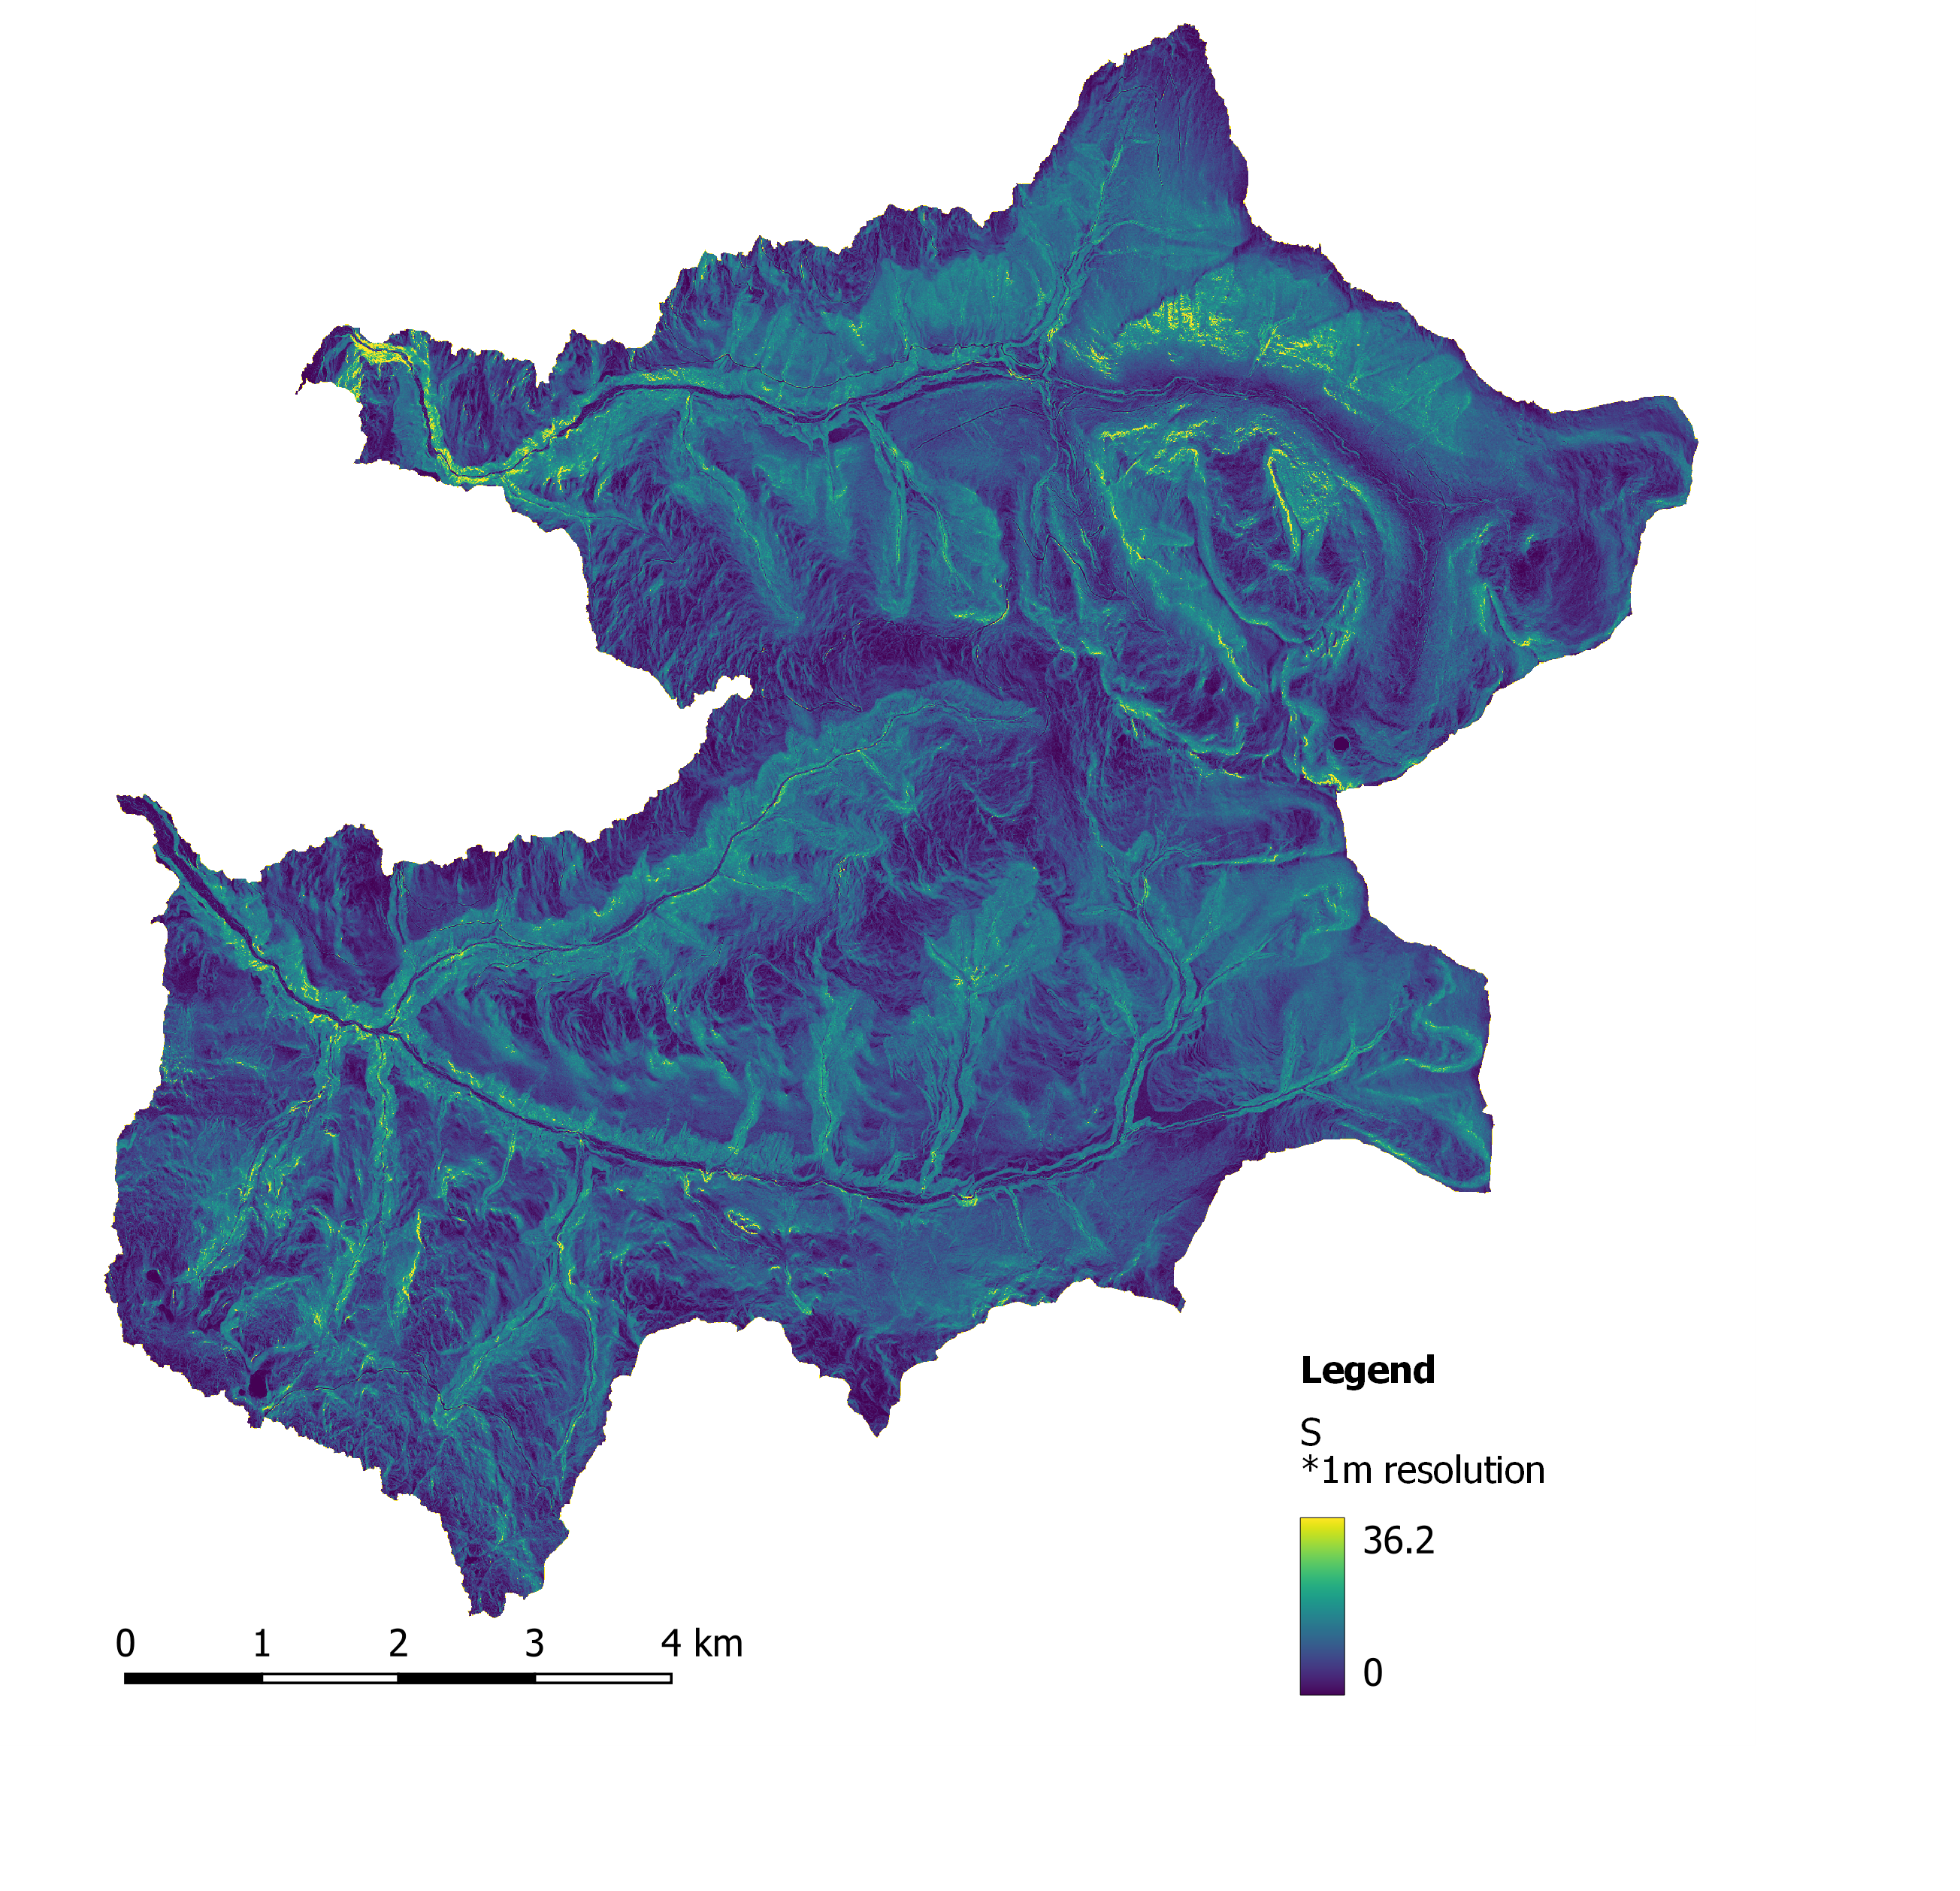
\includegraphics{img/S_1m.png}
\caption{\textbf{Figure 12a}: Slope (S) factor for the Winlaw and Trozzo Creek watersheds. The maximum value in the study area is 36.2 and the minimum value is 0. The resolution is 1m.}
\end{figure}

\begin{figure}
\centering
\includegraphics{img/S_1m_hist.png}
\caption{\textbf{Figure 12a (accompanying histogram)}: Slope factor (S) for the Winlaw and Trozzo Creek watersheds. Pixel value is 1m.}
\end{figure}

\begin{figure}
\centering
\includegraphics{img/S_25m.png}
\caption{\textbf{Figure 12b}: Slope (S) factor for the Winlaw and Trozzo Creek watersheds. The maximum value in the study area is 44.26 and the minimum value is 0. The resolution is 25m.}
\end{figure}

\begin{figure}
\centering
\includegraphics{img/S_25m_hist.png}
\caption{\textbf{Figure 13b (accompanying histogram):} Slope factor (S) for the Winlaw and Trozzo Creek watersheds. Pixel value is 25m.}
\end{figure}

\hypertarget{sec-step-9-ls}{%
\paragraph*{Step 9: LS Factor}\label{sec-step-9-ls}}
\addcontentsline{toc}{paragraph}{Step 9: LS Factor}

The final step for calculating the LS factor is the combination of the \texttt{L} and \texttt{S} raster's produced in Steps 7 and 9 respectively (\textbf{Figure 14a and 14b})).

\begin{Shaded}
\begin{Highlighting}[]
\NormalTok{LS }\OtherTok{=}\NormalTok{ L}\SpecialCharTok{*}\NormalTok{S}
\end{Highlighting}
\end{Shaded}

\begin{figure}
\centering
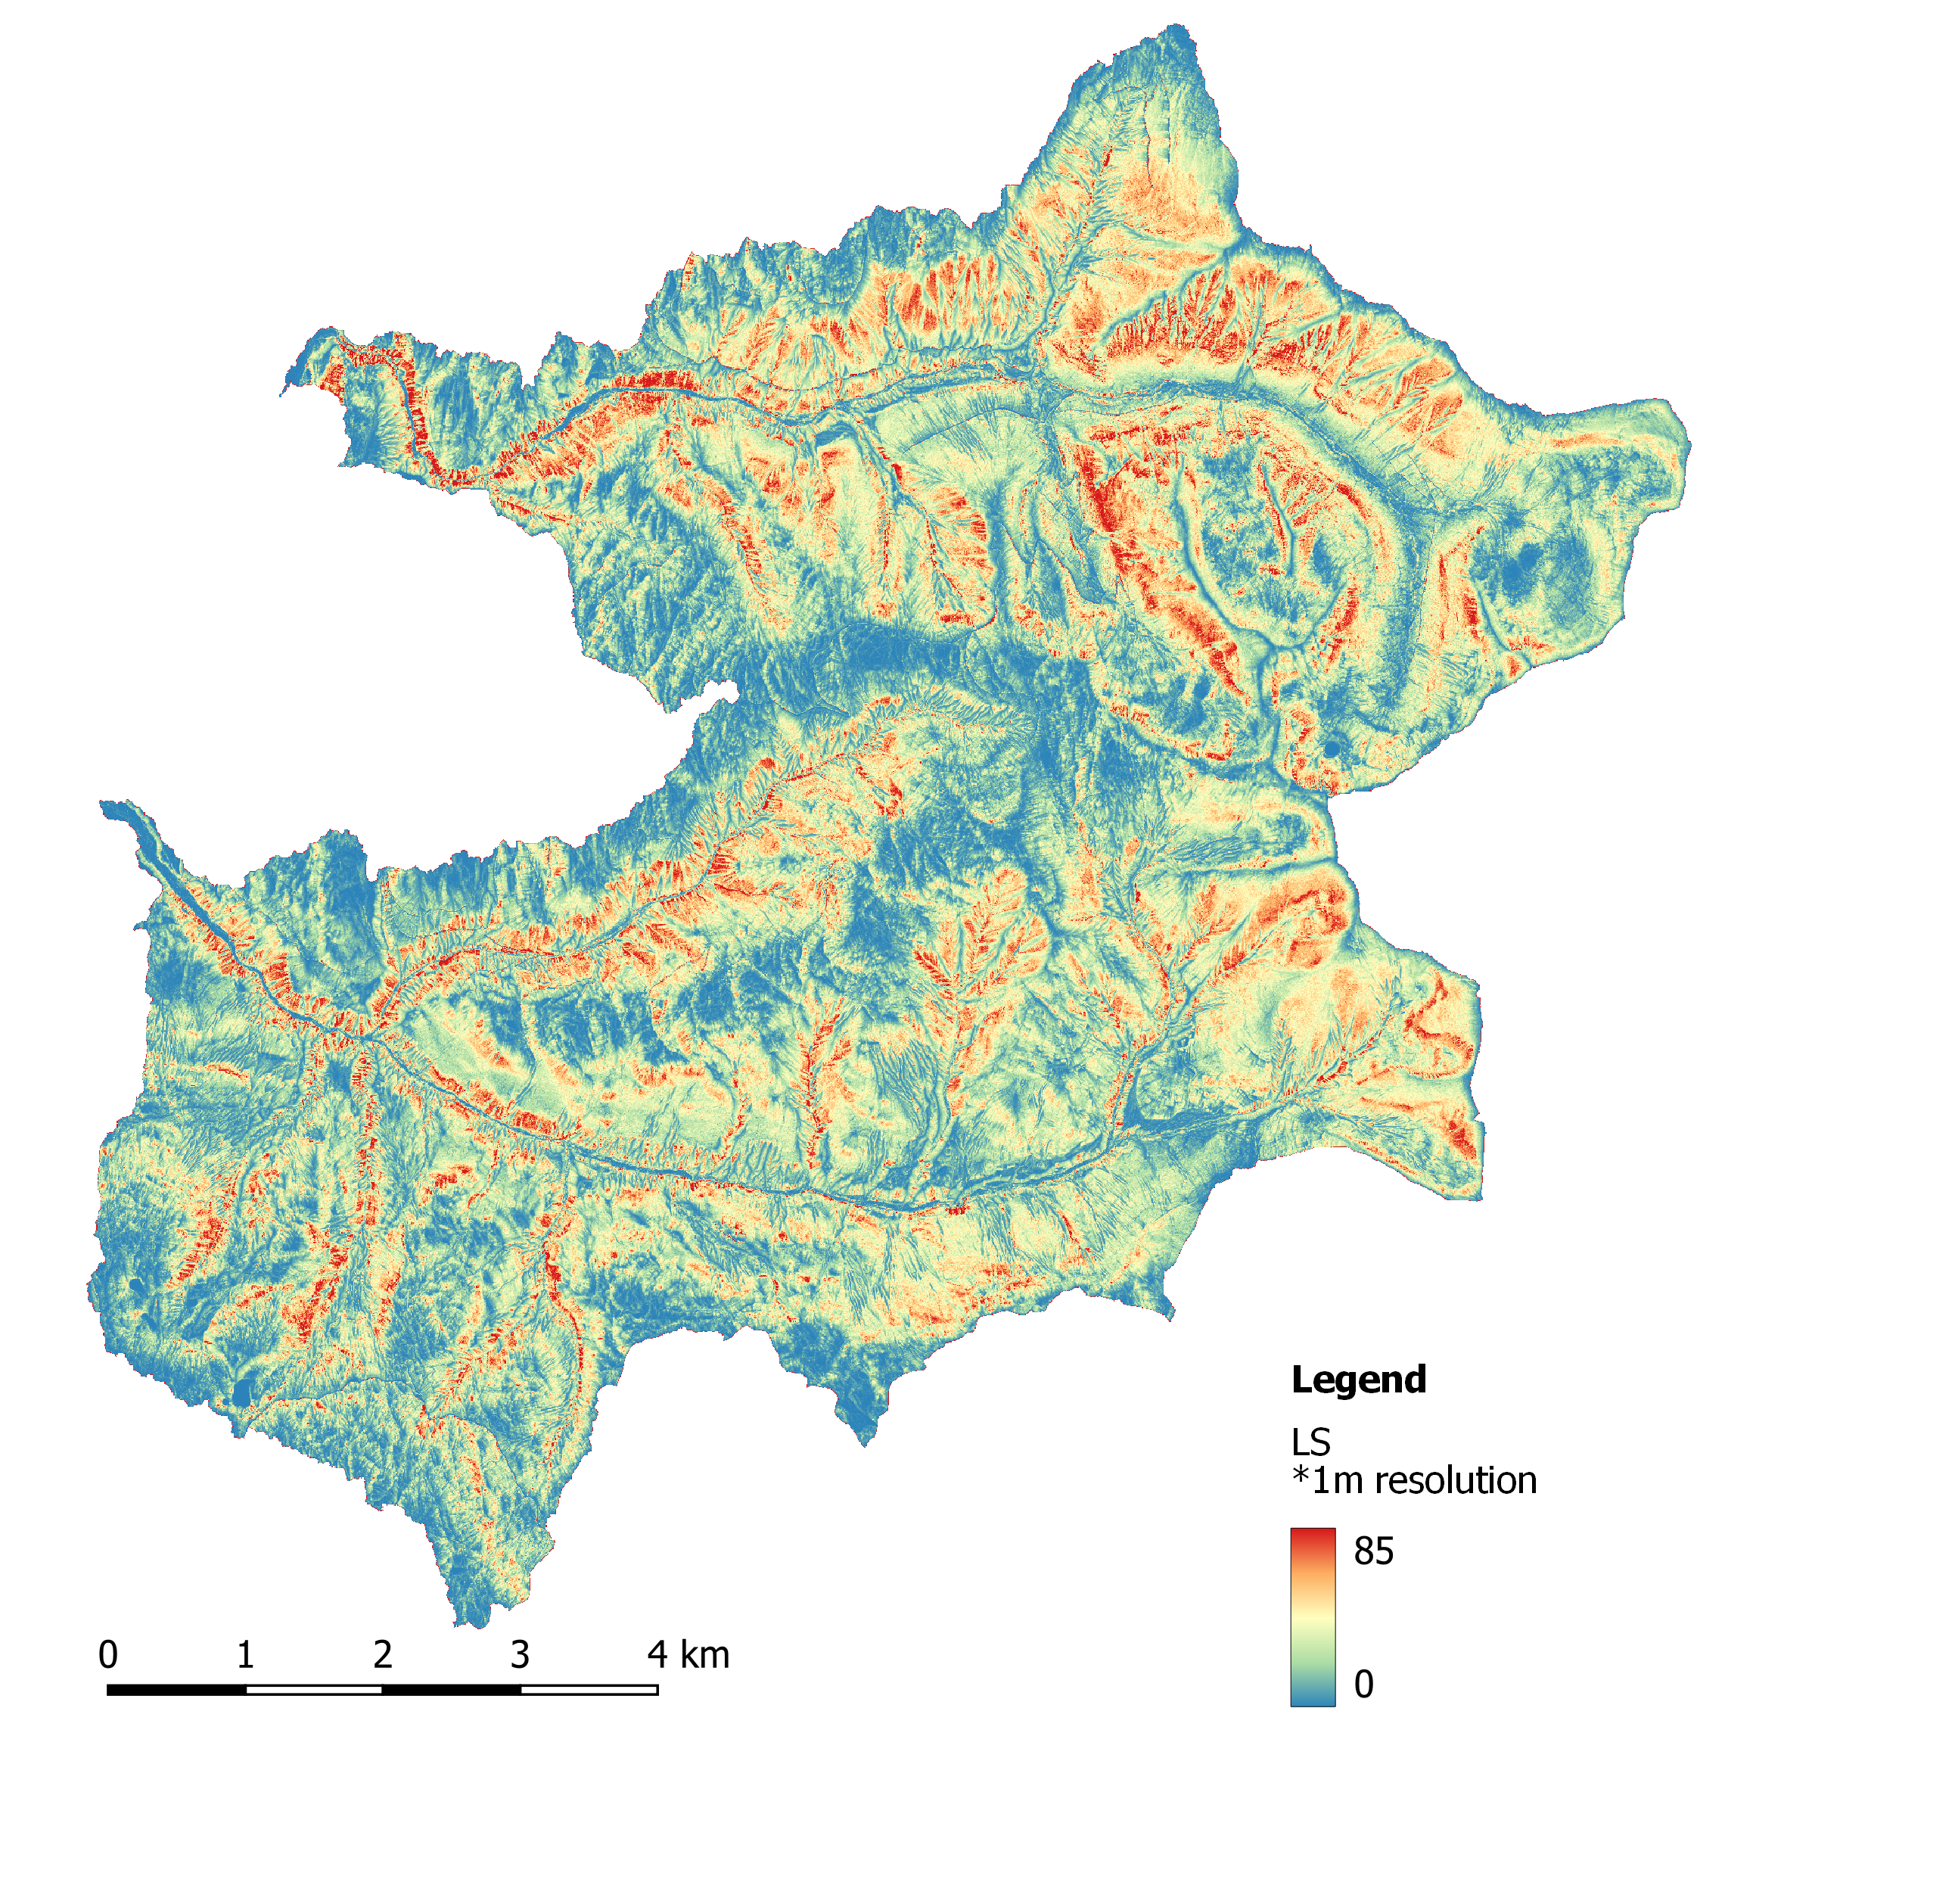
\includegraphics{img/LS_1m.png}
\caption{\textbf{Figure 14a}: Slope Length (LS) factor for the Winlaw and Trozzo Creek watersheds. The maximum value in the study area is 85 and the minimum value is 0. The resolution is 1m.}
\end{figure}

\begin{figure}
\centering
\includegraphics{img/LS_1m_hist.png}
\caption{\textbf{Figure 14a (accompanying histogram)}: Slope Length factor (LS) for the Winlaw and Trozzo Creek watersheds. Pixel value is 1m.}
\end{figure}

\begin{figure}
\centering
\includegraphics{img/LS_25m.png}
\caption{\textbf{Figure 14b}: Slope Length (LS) factor for the Winlaw and Trozzo Creek watersheds. The maximum value in the study area is 43 and the minimum value is 0. The resolution is 25m.}
\end{figure}

\begin{figure}
\centering
\includegraphics{img/LS_25m_hist.png}
\caption{\textbf{Figure 14b (accompanying histogram):} Slope Length factor (LS) for the Winlaw and Trozzo Creek watersheds. Pixel value is 25m}
\end{figure}

\hypertarget{sec-factor-3}{%
\subsection*{Factor 3 - Soil Erodibility (K)}\label{sec-factor-3}}
\addcontentsline{toc}{subsection}{Factor 3 - Soil Erodibility (K)}

\hypertarget{sec-input-data-ls}{%
\subsubsection*{Input Data:}\label{sec-input-data-ls}}
\addcontentsline{toc}{subsubsection}{Input Data:}

K factor (soil erodibility) values are based on values provided by the \href{http://www.omafra.gov.on.ca/english/engineer/facts/12-051.htm}{Ontario Ministry of Agriculture, Food and Rural Affairs} and soil data from the \href{https://catalogue.data.gov.bc.ca/dataset/20150a67-5a2d-425f-8216-ff0f97f68df9}{British Columbia Soil Survey}. These K estimations are based on the information obtained on approximately 1600 samples collected in Southern Ontario by Ontario Institute of Pedology surveyors. Values used here follow the recommendation by \href{https://sis.agr.gc.ca/cansis/publications/manuals/2002-92/rusle-can.pdf}{Wall et al., 2002} (\textbf{Figure 15}). They suggest that if the organic matter content of a soil is unknown and cannot be obtained through extensive soil testing fieldwork, `average K' values should be used for RUSLE modelling.

\includegraphics{img/k_factor_input.png}

\textbf{Figure 15}: Soil Erodibility (K) input data for for the study area located in West Kootenay region of southeastern British Columbia. Data sourced from the Ontario Ministry of Agriculture, Food and Rural Affairs{]}(\url{http://www.omafra.gov.on.ca/english/engineer/facts/12-051.htm}) and soil data from the \href{https://catalogue.data.gov.bc.ca/dataset/20150a67-5a2d-425f-8216-ff0f97f68df9}{British Columbia Soil Survey}.

\hypertarget{sec-calculating-the-k-factor}{%
\subsubsection*{Calculating the K Factor:}\label{sec-calculating-the-k-factor}}
\addcontentsline{toc}{subsubsection}{Calculating the K Factor:}

The first step for calculating K values is to tidy data and determine the average K value by soil texture. There are three soil textures in the study area (according to the \href{https://catalogue.data.gov.bc.ca/dataset/20150a67-5a2d-425f-8216-ff0f97f68df9}{British Columbia Soil Survey}) (\textbf{Table 3}).

\begin{Shaded}
\begin{Highlighting}[]
\NormalTok{trozzo\_soils }\OtherTok{\textless{}{-}} \FunctionTok{read\_sf}\NormalTok{(}\StringTok{"data/4/K/trozzo\_Soils.shp"}\NormalTok{) }\CommentTok{\#BC soils data}
\NormalTok{winlaw\_soils }\OtherTok{\textless{}{-}} \FunctionTok{read\_sf}\NormalTok{(}\StringTok{"data/4/K/winlaw\_Soils.shp"}\NormalTok{) }\CommentTok{\#BC soils data}
\NormalTok{trozzo\_winlaw\_soils }\OtherTok{\textless{}{-}}\FunctionTok{rbind}\NormalTok{(trozzo\_soils, winlaw\_soils) }\CommentTok{\#Combine BC soils data}
\NormalTok{K\_values }\OtherTok{\textless{}{-}} \FunctionTok{read\_excel}\NormalTok{(}\StringTok{"data/4/K/K\_values.xlsx"}\NormalTok{) }\CommentTok{\#Pre{-}determined K values}
\NormalTok{K\_values }\OtherTok{\textless{}{-}} \FunctionTok{subset}\NormalTok{((}\FunctionTok{merge}\NormalTok{(trozzo\_winlaw\_soils, K\_values, }\AttributeTok{by =} \StringTok{"TEXTURE\_1"}\NormalTok{, }\AttributeTok{all.x =} \ConstantTok{TRUE}\NormalTok{)), }\AttributeTok{select =} \FunctionTok{c}\NormalTok{(Average\_K, TEXTURE\_1, AREA\_SQM))}
\end{Highlighting}
\end{Shaded}

\textbf{Table 3.} Soil erodibility values (K) for study area soil textures (Loamy Sand, Silty Loam, Sandy Loam), and the percentage area of soil class per watershed.

\begin{table}
\centering
\begin{tabular}[t]{l|l|r|r}
\hline
Watershed & Soil Texture & Average K Value & Percentage Area (\%)\\
\hline
Trozzo Creek & Loamy Sand & 0.005 & 35.8\\
\hline
 & Silty Loam & 0.017 & 0.2\\
\hline
 & Sandy Loam & 0.050 & 64.0\\
\hline
Winlaw Creek & Loamy Sand & 0.005 & 46.0\\
\hline
 & Silty Loam & 0.017 & 0.0\\
\hline
 & Sandy Loam & 0.050 & 54.0\\
\hline
\end{tabular}
\end{table}

To produce a K value raster (\textbf{Figure 16}), an empty raster must be built using the \texttt{raster} package, this raster will be populated with K values and have the same resolution and extent as the R factor raster:

\begin{Shaded}
\begin{Highlighting}[]
\NormalTok{empty\_raster }\OtherTok{\textless{}{-}} \FunctionTok{reclassify}\NormalTok{(R\_factor, }\FunctionTok{cbind}\NormalTok{(}\DecValTok{0}\NormalTok{, }\DecValTok{800}\NormalTok{, }\DecValTok{0}\NormalTok{), }\AttributeTok{right=}\ConstantTok{FALSE}\NormalTok{)}
\NormalTok{K\_factor }\OtherTok{\textless{}{-}} \FunctionTok{rasterize}\NormalTok{(K\_values, y, }\AttributeTok{field =} \StringTok{"Average\_K"}\NormalTok{, }
                      \AttributeTok{fun =} \StringTok{"max"}\NormalTok{, }\AttributeTok{background =} \FloatTok{0.001}\NormalTok{)}
\NormalTok{empty\_raster }\OtherTok{\textless{}{-}} \FunctionTok{raster}\NormalTok{(}\AttributeTok{ncol =} \DecValTok{11689}\NormalTok{, }\AttributeTok{nrow =} \DecValTok{11737}\NormalTok{ , }
                       \AttributeTok{crs =} \FunctionTok{crs}\NormalTok{(R\_factor), }\AttributeTok{resolution =} \FunctionTok{res}\NormalTok{(R\_factor))}
\FunctionTok{extent}\NormalTok{(empty\_raster) }\OtherTok{\textless{}{-}} \FunctionTok{extent}\NormalTok{(R\_factor)}
\NormalTok{K\_factor }\OtherTok{\textless{}{-}} \FunctionTok{rasterize}\NormalTok{(K\_values, R\_factor, }\AttributeTok{field =} \StringTok{"Average\_K"}\NormalTok{,}
                      \AttributeTok{fun =} \StringTok{"max"}\NormalTok{, }\AttributeTok{background =} \FloatTok{0.001}\NormalTok{)}
\end{Highlighting}
\end{Shaded}

\begin{figure}
\centering
\includegraphics{img/k_factor.png}
\caption{\textbf{Figure 16}: Soil erodibility factor (K) values measured the percentage erodiibilty of soil textures for the Winlaw and Trozzo Creek watershed study areas. The highest K values (max = 0.050) are associated with the Silty Loam soil texture, and the lowest K values (min = 0.005) are associated with the Loamy Sand texture. Data sourced from the British Columbia Soil Survey.}
\end{figure}

\textbf{Figure 16}: Soil erodibility factor (K) values measured the percentage erodiibilty of soil textures for the Winlaw and Trozzo Creek watershed study areas. The highest K values (max = 0.050) are associated with the Silty Loam soil texture, and the lowest K values (min = 0.005) are associated with the Loamy Sand texture. Data sourced from the \href{https://catalogue.data.gov.bc.ca/dataset/20150a67-5a2d-425f-8216-ff0f97f68df9}{British Columbia Soil Survey}.

\hypertarget{sec-factor-4}{%
\subsection*{Factor 4 - Crop/Vegetation and Management Factor}\label{sec-factor-4}}
\addcontentsline{toc}{subsection}{Factor 4 - Crop/Vegetation and Management Factor}

\hypertarget{sec-input-data-c}{%
\subsubsection*{Input Data:}\label{sec-input-data-c}}
\addcontentsline{toc}{subsubsection}{Input Data:}

There are no current, or recorded soil erosion management practices being implemented in the study area. Therefore the C factor is is based on:

\begin{enumerate}
\def\labelenumi{\arabic{enumi}.}
\tightlist
\item
  Vegetation cover, specified by the \href{https://www2.gov.bc.ca/gov/content/industry/forestry/managing-our-forest-resources/forest-inventory}{Vegetation Resource Inventory(VRI)} (\textbf{Figure 17})) .
\end{enumerate}

\includegraphics{img/c_factor_input_vri.png}

\textbf{Figure 17} Crop/Vegetation and Management Factor (C) Vegetation Resource Inventory (VRI) data for for the study area located in West Kootenay region of southeastern British Columbia. Data sourced from the \href{https://www2.gov.bc.ca/gov/content/industry/forestry/managing-our-forest-resources/forest-inventory}{Vegetation Resource Inventory (VRI)}.

\begin{enumerate}
\def\labelenumi{\arabic{enumi}.}
\setcounter{enumi}{1}
\tightlist
\item
  Fire Burn Severity, specified by provincial \href{https://catalogue.data.gov.bc.ca/dataset/fire-burn-severity-historical}{Burn Severity Mapping} completed using Landsat or Satellite imagery (\textbf{Figure 18}).
\end{enumerate}

\includegraphics{img/c_factor_input_bs.png}

\textbf{Figure 18}: Crop/Vegetation and Management Factor (C) Burn Severity Mapping data for for the study area located in West Kootenay region of southeastern British Columbia. Data sourced from BC \href{https://catalogue.data.gov.bc.ca/dataset/fire-burn-severity-historical}{Burn Severity Mapping} completed using Landsat or Satellite imagery.

\begin{enumerate}
\def\labelenumi{\arabic{enumi}.}
\setcounter{enumi}{2}
\tightlist
\item
  Road network, sourced from the provincial \href{https://www2.gov.bc.ca/gov/content/data/geographic-data-services/topographic-data/roads}{Digital Road Atlas} (\textbf{Figure 19})
\end{enumerate}

\includegraphics{img/c_factor_input_roads10m.png}\{

\textbf{Figure 19}: Crop/Vegetation and Management Factor (C) Road data for for the study area located in West Kootenay region of southeastern British Columbia. Data sourced from BC \href{https://www2.gov.bc.ca/gov/content/data/geographic-data-services/topographic-data/roads}{Digital Road Atlas} and bufferd to 10m.

\hypertarget{sec-calculating-the-c-factor}{%
\subsubsection*{Calculating the C Factor:}\label{sec-calculating-the-c-factor}}
\addcontentsline{toc}{subsubsection}{Calculating the C Factor:}

C Factor values are assigned to each Crop/Vegetation and Management input, and vary depending on the impact (Table \ref{tab:4}).

\textbf{Table 4}: Crop/Vegetation and Management values (K) for the study area for Vegetation Resource Inventory (VRI) class, Burn Severity, and Road presence.

\begin{table}
\centering
\begin{tabular}[t]{l|r}
\hline
C Factor Class & C Factor Value\\
\hline
Burn Severity - High & 0.20\\
\hline
Burn Severity - Medium & 0.05\\
\hline
Burn Severity - Low & 0.01\\
\hline
VRI - Treed & 0.01\\
\hline
VRI - Herb & 0.01\\
\hline
VRI - Shrub & 0.01\\
\hline
VRI - Rock & 0.20\\
\hline
VRI - Exposed Land & 0.01\\
\hline
Roads & 0.20\\
\hline
\end{tabular}
\end{table}

Calculating the C factor involves seven steps:

\hypertarget{sec-step-1-reclassifying-vri-data-c}{%
\paragraph*{Step 1: Reclassifying VRI Data}\label{sec-step-1-reclassifying-vri-data-c}}
\addcontentsline{toc}{paragraph}{Step 1: Reclassifying VRI Data}

\begin{Shaded}
\begin{Highlighting}[]
\NormalTok{vri\_data }\OtherTok{\textless{}{-}} \FunctionTok{st\_read}\NormalTok{(}\StringTok{"data/VRI.shp"}\NormalTok{)}
\NormalTok{vri\_data[}\StringTok{\textquotesingle{}C\_Factor\textquotesingle{}}\NormalTok{] }\OtherTok{=} \FunctionTok{as.numeric}\NormalTok{()}

\NormalTok{vri\_data }\SpecialCharTok{\%\textgreater{}\%}
  \FunctionTok{mutate}\NormalTok{(}\AttributeTok{C\_Factor =} \FunctionTok{case\_when}\NormalTok{(}
    \FunctionTok{endsWith}\NormalTok{(BCLCS\_LV\_4, }\StringTok{"HE"}\NormalTok{) }\SpecialCharTok{\textasciitilde{}} \FunctionTok{as.numeric}\NormalTok{(}\FloatTok{0.01}\NormalTok{), }
    \FunctionTok{endsWith}\NormalTok{(BCLCS\_LV\_4, }\StringTok{"TB"}\NormalTok{) }\SpecialCharTok{\textasciitilde{}} \FunctionTok{as.numeric}\NormalTok{(}\FloatTok{0.01}\NormalTok{), }
    \FunctionTok{endsWith}\NormalTok{(BCLCS\_LV\_4, }\StringTok{"TM"}\NormalTok{) }\SpecialCharTok{\textasciitilde{}} \FunctionTok{as.numeric}\NormalTok{(}\FloatTok{0.01}\NormalTok{), }
    \FunctionTok{endsWith}\NormalTok{(BCLCS\_LV\_4, }\StringTok{"SL"}\NormalTok{) }\SpecialCharTok{\textasciitilde{}} \FunctionTok{as.numeric}\NormalTok{(}\FloatTok{0.01}\NormalTok{), }
    \FunctionTok{endsWith}\NormalTok{(BCLCS\_LV\_4, }\StringTok{"EL"}\NormalTok{) }\SpecialCharTok{\textasciitilde{}} \FunctionTok{as.numeric}\NormalTok{(}\FloatTok{0.01}\NormalTok{), }
    \FunctionTok{endsWith}\NormalTok{(BCLCS\_LV\_4, }\StringTok{"TC"}\NormalTok{) }\SpecialCharTok{\textasciitilde{}} \FunctionTok{as.numeric}\NormalTok{(}\FloatTok{0.01}\NormalTok{), }
    \FunctionTok{endsWith}\NormalTok{(BCLCS\_LV\_4, }\StringTok{"RO"}\NormalTok{) }\SpecialCharTok{\textasciitilde{}} \FunctionTok{as.numeric}\NormalTok{(}\FloatTok{0.2}\NormalTok{),}
    \FunctionTok{endsWith}\NormalTok{(BCLCS\_LV\_4, }\StringTok{"ST"}\NormalTok{) }\SpecialCharTok{\textasciitilde{}} \FunctionTok{as.numeric}\NormalTok{(}\FloatTok{0.01}\NormalTok{), }
    \FunctionTok{endsWith}\NormalTok{(BCLCS\_LV\_3, }\StringTok{"W"}\NormalTok{) }\SpecialCharTok{\textasciitilde{}} \FunctionTok{as.numeric}\NormalTok{(}\FloatTok{0.01}\NormalTok{)}
\NormalTok{    ))}
\end{Highlighting}
\end{Shaded}

\hypertarget{sec-step-2-reclassifying-burn-severity-data-c}{%
\paragraph*{Step 2: Reclassifying Burn Severity Data}\label{sec-step-2-reclassifying-burn-severity-data-c}}
\addcontentsline{toc}{paragraph}{Step 2: Reclassifying Burn Severity Data}

\begin{Shaded}
\begin{Highlighting}[]
\NormalTok{BurnSeverity }\OtherTok{\textless{}{-}} \FunctionTok{st\_read}\NormalTok{(}\StringTok{"data/BurnSeverity.shp"}\NormalTok{)}
\NormalTok{BurnSeverity[}\StringTok{\textquotesingle{}C\_Factor\textquotesingle{}}\NormalTok{] }\OtherTok{=} \FunctionTok{as.numeric}\NormalTok{()}

\NormalTok{BurnSeverity }\SpecialCharTok{\%\textgreater{}\%}
  \FunctionTok{mutate}\NormalTok{(}\AttributeTok{C\_Factor =} \FunctionTok{case\_when}\NormalTok{(}
    \FunctionTok{endsWith}\NormalTok{(BurnSev, }\StringTok{"High"}\NormalTok{) }\SpecialCharTok{\textasciitilde{}} \FunctionTok{as.numeric}\NormalTok{(}\FloatTok{0.2}\NormalTok{), }
    \FunctionTok{endsWith}\NormalTok{(BurnSev, }\StringTok{"Low"}\NormalTok{) }\SpecialCharTok{\textasciitilde{}} \FunctionTok{as.numeric}\NormalTok{(}\FloatTok{0.01}\NormalTok{), }
    \FunctionTok{endsWith}\NormalTok{(BurnSev, }\StringTok{"Medium"}\NormalTok{) }\SpecialCharTok{\textasciitilde{}} \FunctionTok{as.numeric}\NormalTok{(}\FloatTok{0.05}\NormalTok{)}
\NormalTok{    ))}
\end{Highlighting}
\end{Shaded}

\hypertarget{step-3-reclassifying-and-buffering-road-data}{%
\paragraph*{Step 3: Reclassifying and Buffering Road Data}\label{step-3-reclassifying-and-buffering-road-data}}
\addcontentsline{toc}{paragraph}{Step 3: Reclassifying and Buffering Road Data}

\begin{Shaded}
\begin{Highlighting}[]
\NormalTok{roads\_buff\_10 }\OtherTok{\textless{}{-}} \FunctionTok{st\_buffer}\NormalTok{(roads, }\DecValTok{10}\NormalTok{)}
\NormalTok{roads\_buff\_10}\SpecialCharTok{$}\NormalTok{C\_Factor }\OtherTok{\textless{}{-}} \FloatTok{0.2}
\end{Highlighting}
\end{Shaded}

\hypertarget{sec-step-3-vri-polygon-to-raster-c}{%
\paragraph*{Step 4: VRI Polygon to Raster}\label{sec-step-3-vri-polygon-to-raster-c}}
\addcontentsline{toc}{paragraph}{Step 4: VRI Polygon to Raster}

\begin{Shaded}
\begin{Highlighting}[]
\NormalTok{vri\_data\_spdf }\OtherTok{\textless{}{-}} \FunctionTok{as\_Spatial}\NormalTok{(vri\_data)}
\NormalTok{empty\_raster }\OtherTok{\textless{}{-}}\FunctionTok{raster}\NormalTok{(}\AttributeTok{res =} \DecValTok{1}\NormalTok{, }\AttributeTok{ext =}\NormalTok{ extent)}
\FunctionTok{crs}\NormalTok{(empty\_raster) }\OtherTok{\textless{}{-}} \FunctionTok{crs}\NormalTok{(LS\_1m)}
\NormalTok{vri }\OtherTok{\textless{}{-}} \FunctionTok{rasterize}\NormalTok{(vri\_data, empty\_raster, }\AttributeTok{field =} \StringTok{"C\_Factor"}\NormalTok{, }\AttributeTok{res =} \DecValTok{1}\NormalTok{)}
\end{Highlighting}
\end{Shaded}

\hypertarget{sec-step-5-burn-severity-polygon-to-raster}{%
\paragraph*{Step 5: Burn Severity Polygon to Raster}\label{sec-step-5-burn-severity-polygon-to-raster}}
\addcontentsline{toc}{paragraph}{Step 5: Burn Severity Polygon to Raster}

\begin{Shaded}
\begin{Highlighting}[]
\NormalTok{BurnSeverity\_spdf }\OtherTok{\textless{}{-}} \FunctionTok{as\_Spatial}\NormalTok{(BurnSeverity)}
\NormalTok{empty\_raster }\OtherTok{\textless{}{-}}\FunctionTok{raster}\NormalTok{(}\AttributeTok{res =} \DecValTok{1}\NormalTok{, }\AttributeTok{ext =}\NormalTok{ extent)}
\FunctionTok{crs}\NormalTok{(empty\_raster) }\OtherTok{\textless{}{-}} \FunctionTok{crs}\NormalTok{(LS\_1m)}
\NormalTok{burn }\OtherTok{\textless{}{-}} \FunctionTok{rasterize}\NormalTok{(BurnSeverity, empty\_raster, }\AttributeTok{field =} \StringTok{"C\_Factor"}\NormalTok{)}
\end{Highlighting}
\end{Shaded}

\hypertarget{sec-step-5-road-polygon-to-raster-c}{%
\paragraph*{Step 6: Road Polygon to Raster}\label{sec-step-5-road-polygon-to-raster-c}}
\addcontentsline{toc}{paragraph}{Step 6: Road Polygon to Raster}

\begin{Shaded}
\begin{Highlighting}[]
\NormalTok{roads\_data\_spdf }\OtherTok{\textless{}{-}} \FunctionTok{as\_Spatial}\NormalTok{(roads\_buff\_10)}
\NormalTok{empty\_raster }\OtherTok{\textless{}{-}}\FunctionTok{raster}\NormalTok{(}\AttributeTok{res =} \DecValTok{1}\NormalTok{, }\AttributeTok{ext =}\NormalTok{ extent)}
\FunctionTok{crs}\NormalTok{(empty\_raster) }\OtherTok{\textless{}{-}} \FunctionTok{crs}\NormalTok{(LS\_1m)}
\NormalTok{roads }\OtherTok{\textless{}{-}} \FunctionTok{rasterize}\NormalTok{(roads\_buff\_10, empty\_raster, }\AttributeTok{field =} \StringTok{"C\_Factor"}\NormalTok{, }\AttributeTok{res =} \DecValTok{1}\NormalTok{)}
\end{Highlighting}
\end{Shaded}

\hypertarget{sec-step-6-c-factor-c}{%
\paragraph*{Step 7: C Factor}\label{sec-step-6-c-factor-c}}
\addcontentsline{toc}{paragraph}{Step 7: C Factor}

\begin{Shaded}
\begin{Highlighting}[]
\NormalTok{C\_Factor\_Post\_Fire }\OtherTok{\textless{}{-}} \FunctionTok{mosaic}\NormalTok{(vri, roads, }\AttributeTok{fun =} \StringTok{"max"}\NormalTok{, }\AttributeTok{tolerance =} \FloatTok{0.2}\NormalTok{)}
\NormalTok{C\_Factor\_Pre\_Fire }\OtherTok{\textless{}{-}} \FunctionTok{mosaic}\NormalTok{(vri, roads, }\AttributeTok{fun =} \StringTok{"max"}\NormalTok{, }\AttributeTok{tolerance =} \FloatTok{0.2}\NormalTok{)}
\end{Highlighting}
\end{Shaded}

This project is concerned with soil erosion modeling in a region which experienced a large fire. To that end, we produce two C Factor rasters, one pre-burn (\textbf{Figure 20}) and one post-burn (\textbf{Figure 21}).

\includegraphics{img/c_factor_pre_burn_roads10m.png}\}

\textbf{Figure 20:} Pre-burn Crop/Vegetation and Management Factor (C) for the Winlaw and Trozzo Creek watershed study areas.

\includegraphics{img/c_factor_post_burn_roads10m.png}

\textbf{Figure 21}: Post-burn Crop/Vegetation and Management Factor (C) for the Winlaw and Trozzo Creek watershed study areas.

\hypertarget{sec-applying-the-rusle-equation}{%
\section*{Applying the RUSLE Equation:}\label{sec-applying-the-rusle-equation}}
\addcontentsline{toc}{section}{Applying the RUSLE Equation:}

In this section, we show two example applications of the RUSLE. These case studies highlight applications of the RUSLE in the same region pre and post-fire.

\hypertarget{sec-application-1-rusle-post-burn}{%
\subsection*{Application 1: RUSLE Post Burn}\label{sec-application-1-rusle-post-burn}}
\addcontentsline{toc}{subsection}{Application 1: RUSLE Post Burn}

\hypertarget{sec-step-1-load-rusle-factors}{%
\subsubsection*{Step 1: Load RUSLE Factors}\label{sec-step-1-load-rusle-factors}}
\addcontentsline{toc}{subsubsection}{Step 1: Load RUSLE Factors}

\begin{Shaded}
\begin{Highlighting}[]
\NormalTok{K }\OtherTok{=} \FunctionTok{raster}\NormalTok{(}\StringTok{"data/4/K/K\_Factor.tif"}\NormalTok{)}
\NormalTok{R }\OtherTok{=} \FunctionTok{raster}\NormalTok{(}\StringTok{"data/4/R/R\_Factor.tif"}\NormalTok{)}
\NormalTok{LS }\OtherTok{=} \FunctionTok{raster}\NormalTok{(}\StringTok{"data/4/LS/LS\_Factor.tif"}\NormalTok{)}
\NormalTok{C\_PreBurn }\OtherTok{=} \FunctionTok{raster}\NormalTok{(}\StringTok{"data/4/C/C\_Factor\_PreBurn.tif"}\NormalTok{)}
\end{Highlighting}
\end{Shaded}

\hypertarget{sec-step-3-re-sample-rusle-factors}{%
\subsubsection*{Step 2: Re-sample RUSLE Factors}\label{sec-step-3-re-sample-rusle-factors}}
\addcontentsline{toc}{subsubsection}{Step 2: Re-sample RUSLE Factors}

\begin{Shaded}
\begin{Highlighting}[]
\NormalTok{K }\OtherTok{\textless{}{-}}  \FunctionTok{resample}\NormalTok{(K, LS)}
\NormalTok{R }\OtherTok{\textless{}{-}}  \FunctionTok{resample}\NormalTok{(R, LS)}
\NormalTok{C }\OtherTok{\textless{}{-}}  \FunctionTok{resample}\NormalTok{(C, LS)}
\NormalTok{C\_PreBurn }\OtherTok{\textless{}{-}}  \FunctionTok{resample}\NormalTok{(C\_PreBurn, LS)}
\end{Highlighting}
\end{Shaded}

\hypertarget{sec-step-4-combine-factors-using-the-rusle}{%
\subsubsection*{Step 3: Combine Factors using the RUSLE}\label{sec-step-4-combine-factors-using-the-rusle}}
\addcontentsline{toc}{subsubsection}{Step 3: Combine Factors using the RUSLE}

\begin{Shaded}
\begin{Highlighting}[]
\NormalTok{RUSLE\_PreBurn }\OtherTok{\textless{}{-}}\NormalTok{ LS}\SpecialCharTok{*}\NormalTok{K}\SpecialCharTok{*}\NormalTok{R}\SpecialCharTok{*}\NormalTok{C\_PreBurn}
\end{Highlighting}
\end{Shaded}

\begin{figure}
\centering
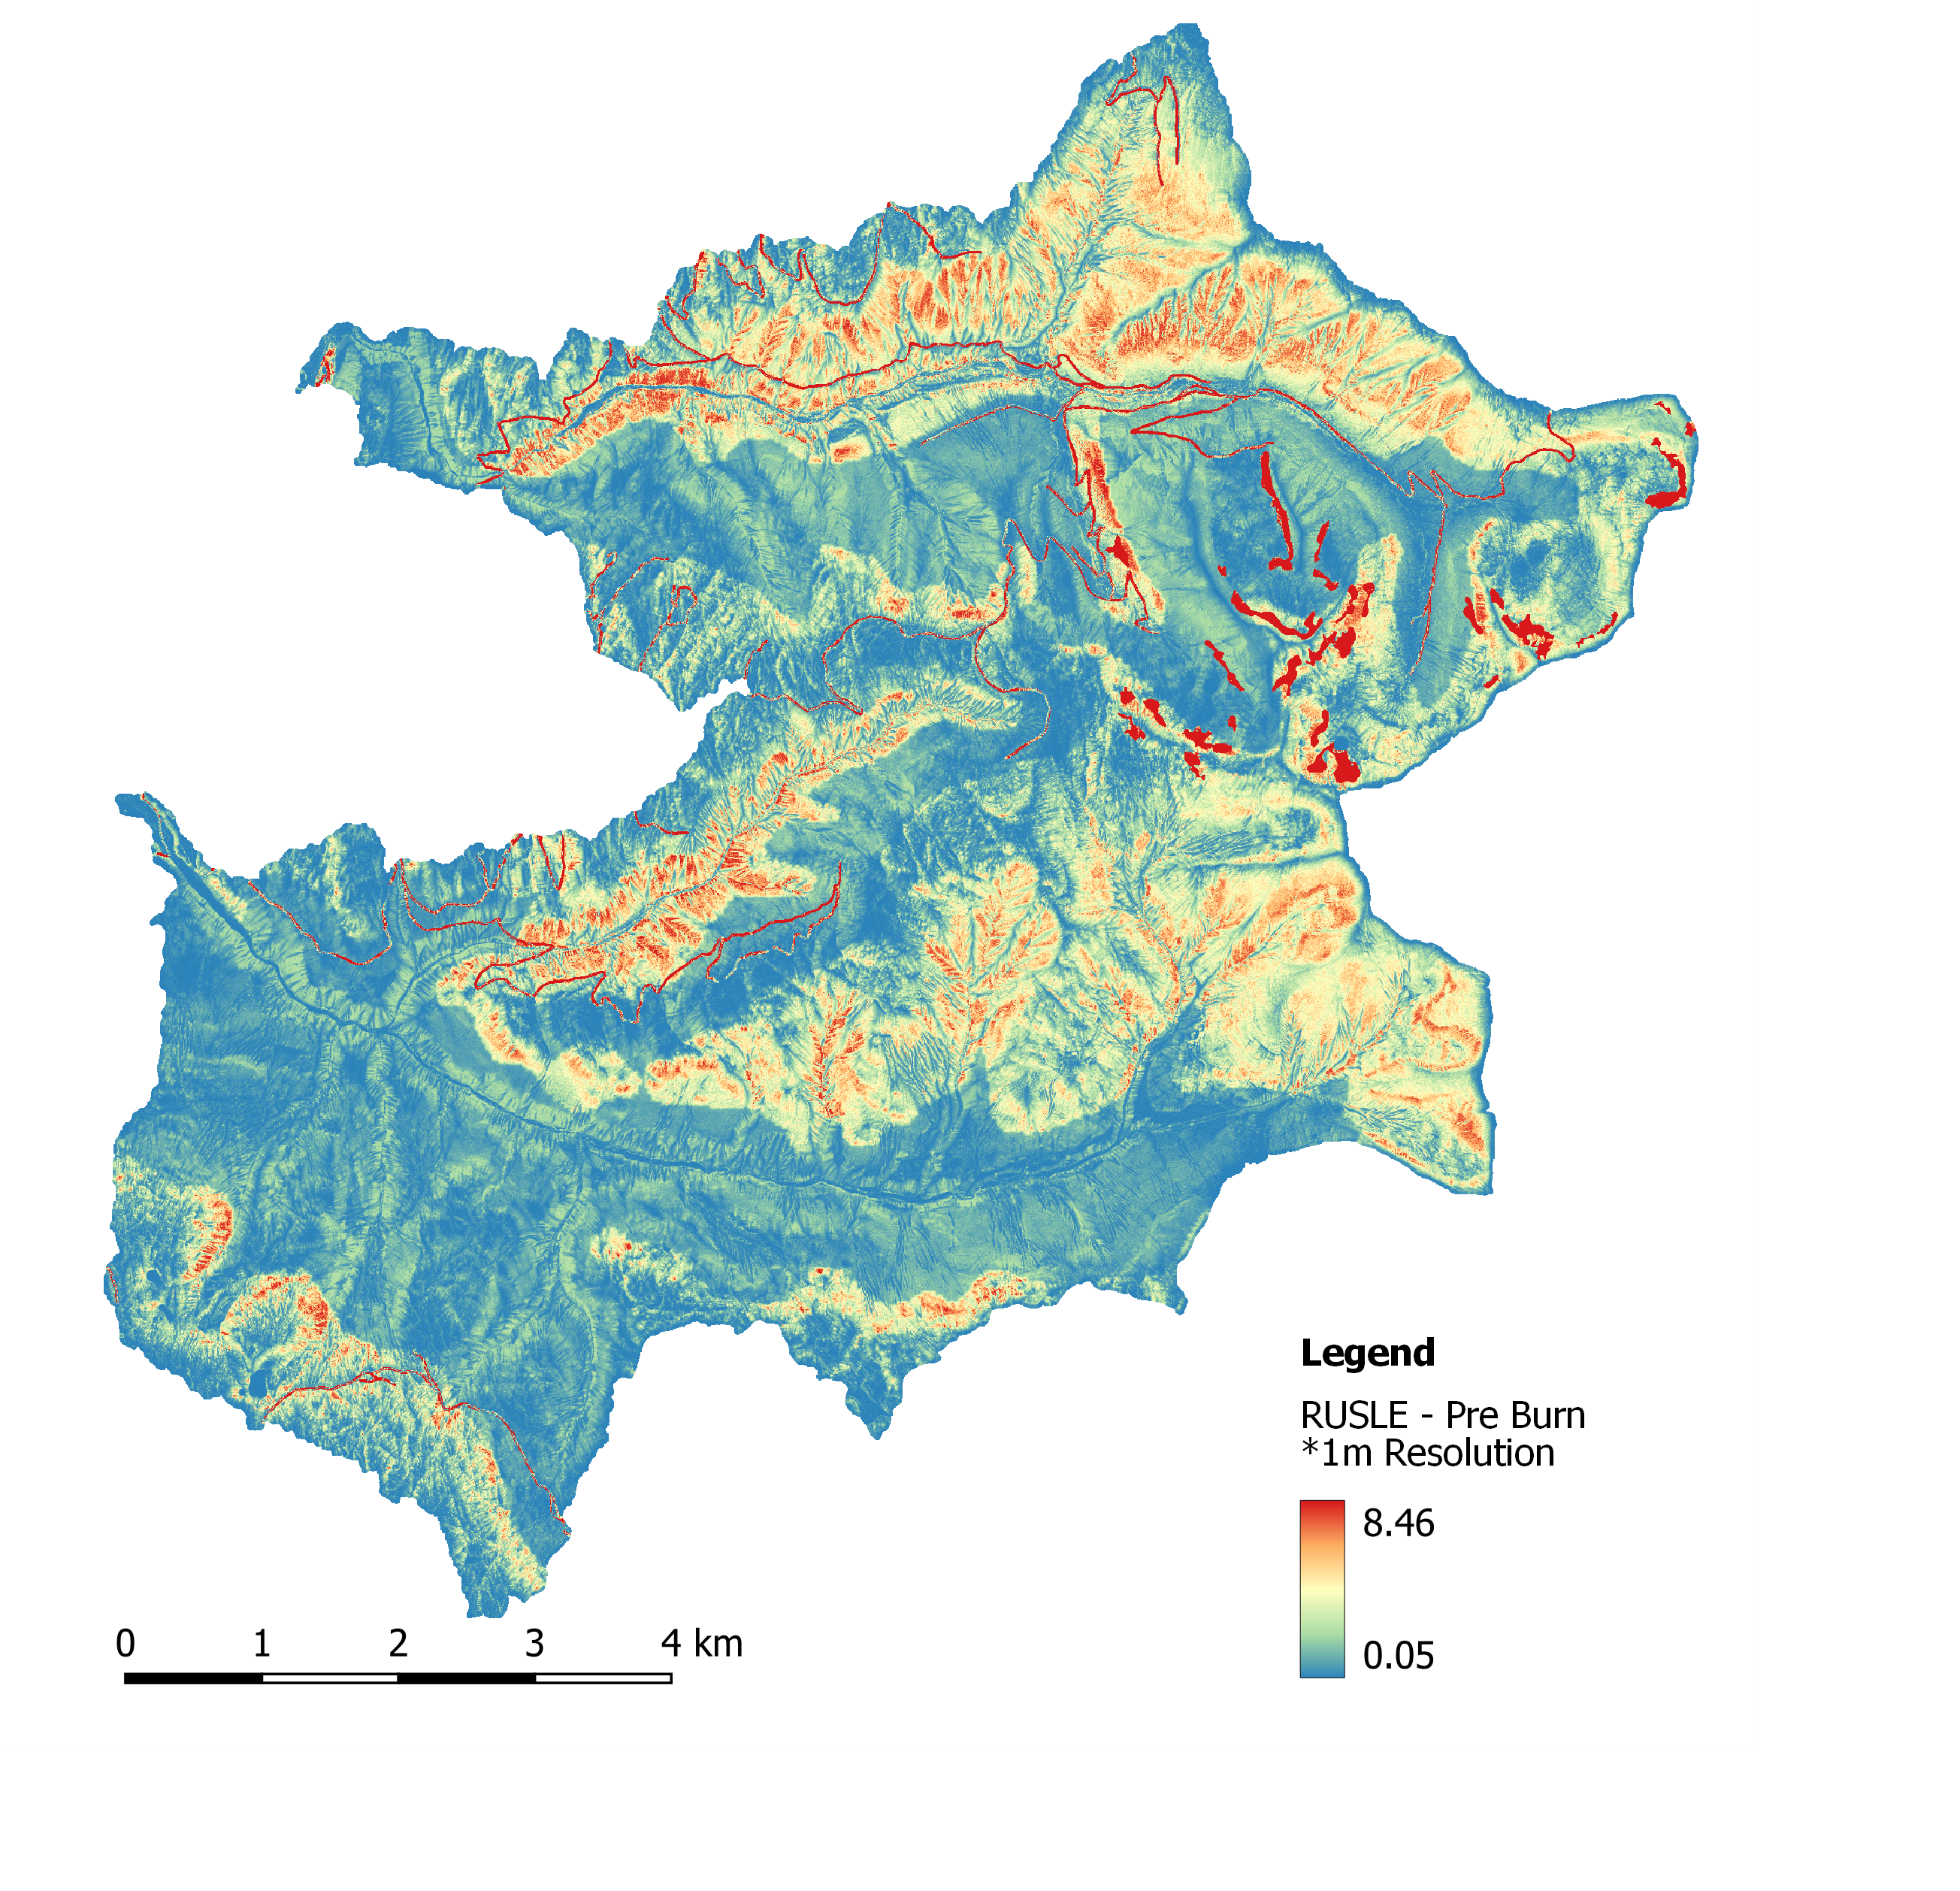
\includegraphics{img/rusle_1m_pretfire.png}
\caption{\textbf{Figure 22:} Pre Burn RUSLE map for the study area located in West Kootenay region of southeastern British Columbia. The resolution is 1m.}
\end{figure}

\begin{figure}
\centering
\includegraphics{img/rusle_25m_prefire.png}
\caption{\textbf{Figure 23:} Pre Burn RUSLE map for the study area located in West Kootenay region of southeastern British Columbia. The resolution is 25m.}
\end{figure}

\hypertarget{sec-application-2-rusle-post-burn}{%
\subsection*{Application 2: RUSLE Post Burn}\label{sec-application-2-rusle-post-burn}}
\addcontentsline{toc}{subsection}{Application 2: RUSLE Post Burn}

\hypertarget{sec-step-1-load-rusle-factors_post}{%
\subsubsection*{Step 1: Load RUSLE Factors}\label{sec-step-1-load-rusle-factors_post}}
\addcontentsline{toc}{subsubsection}{Step 1: Load RUSLE Factors}

\begin{Shaded}
\begin{Highlighting}[]
\NormalTok{K }\OtherTok{=} \FunctionTok{raster}\NormalTok{(}\StringTok{"data/4/K/K\_Factor.tif"}\NormalTok{)}
\NormalTok{R }\OtherTok{=} \FunctionTok{raster}\NormalTok{(}\StringTok{"data/4/R/R\_Factor.tif"}\NormalTok{)}
\NormalTok{LS }\OtherTok{=} \FunctionTok{raster}\NormalTok{(}\StringTok{"data/4/LS/LS\_Factor.tif"}\NormalTok{)}
\NormalTok{C\_PostBurn }\OtherTok{=} \FunctionTok{raster}\NormalTok{(}\StringTok{"data/4/C/C\_Factor\_PostBurn.tif"}\NormalTok{)}
\end{Highlighting}
\end{Shaded}

\hypertarget{sec-step-3-resample-rusle-factors}{%
\subsubsection*{Step 2: Re-sample RUSLE Factors}\label{sec-step-3-resample-rusle-factors}}
\addcontentsline{toc}{subsubsection}{Step 2: Re-sample RUSLE Factors}

\begin{Shaded}
\begin{Highlighting}[]
\NormalTok{K }\OtherTok{\textless{}{-}}  \FunctionTok{resample}\NormalTok{(K, LS)}
\NormalTok{R }\OtherTok{\textless{}{-}}  \FunctionTok{resample}\NormalTok{(R, LS)}
\NormalTok{C }\OtherTok{\textless{}{-}}  \FunctionTok{resample}\NormalTok{(C, LS)}
\NormalTok{C\_PostBurn }\OtherTok{\textless{}{-}}  \FunctionTok{resample}\NormalTok{(C\_PostBurn, LS)}
\end{Highlighting}
\end{Shaded}

\hypertarget{sec-step-4-combine-factors-using-the-rusle-post}{%
\subsubsection*{Step 3: Combine Factors using the RUSLE}\label{sec-step-4-combine-factors-using-the-rusle-post}}
\addcontentsline{toc}{subsubsection}{Step 3: Combine Factors using the RUSLE}

\begin{Shaded}
\begin{Highlighting}[]
\NormalTok{RUSLE\_PostBurn }\OtherTok{\textless{}{-}}\NormalTok{ LS}\SpecialCharTok{*}\NormalTok{K}\SpecialCharTok{*}\NormalTok{R}\SpecialCharTok{*}\NormalTok{C\_PostBurn}
\end{Highlighting}
\end{Shaded}

\begin{figure}
\centering
\includegraphics{img/rusle_1m_postfire.png}
\caption{\textbf{Figure 24:} Post Burn RUSLE map for the study area located in West Kootenay region of southeastern British Columbia. The resolution is 1m.}
\end{figure}

\begin{figure}
\centering
\includegraphics{img/rusle_25m_postfire.png}
\caption{\textbf{Figure 25:} Post Burn RUSLE map for the study area located in West Kootenay region of southeastern British Columbia. The resolution is 25m.}
\end{figure}

\end{document}
